\chapter{Data-driven Networking}
Once we have any computer network as described above, we have a good basis for not only allowing two machines to communicate with one another, but also to do so \emph{efficiently}.
That isn't to say that there is no room to improve on how networks and operating systems provide this functionality.
Many aspects of modern networks, such as \glspl{acr:cca}, thresholds for differentiating services, and flow classification rely heavily upon hand-tuned heuristics.
As in \cref{sec:problems-in-modern-networks}, there is still vast scope to improve on communication latency and throughput, or to avoid and work around deleterious traffic patterns (such as incast communication).
As a result, research into \glspl{acr:cca}, network designs, and routing procedures is very much ongoing.
Crucially, as these operations lie at the core of network operation their solutions tend towards extremely efficient heuristic methods; they must be evaluated per-packet or react as quickly as possible to state change.
Designing new methods for network optimisation then requires deep insight into any problem, its edge cases, and the hardware/performance characteristics of the target environment.\sidenote{This affects how we design such heuristics even on commodity hosts---for instance, kernel-space \glspl{acr:cca} (i.e., as part of the TCP stack) are unable to use floating point arithmetic.}

Suppose that, as network administrators or protocol designers, we have access to a reasonable amount of information about the machines, network segments or \glspl{acr:as} under our control---measurements, observations, and statistics taken at run-time, from simulation, or by modelling.
A natural question to ask, then, is whether we can use this data to enhance and improve the operation and use of our network automatically.
Thinking further still, we might wonder whether we can outperform the general (yet useful) heuristics which are widely deployed and researched, allowing us to tailor network behaviour according to its environment and traffic patterns.
These questions are the founding principles of \gls{acr:ddn}\sidenote{Alternatively titled \emph{self-driving networks}.}, a recent field of research focussed on the automatic control and optimisation of network systems, which has sprung forth due to recent advances in \gls{acr:ml} and \gls{acr:rl}~\parencite{DBLP:conf/anrw/FeamsterR18,DBLP:journals/pieee/KellererKBBR019}.

The ideas and goals of automated network control have always existed and evolved in one form or another, particularly as computational inference and learning have grown more powerful.
Primarily, these ideas have propagated in their early forms via position papers offering a `vision of things to come'.
This was first famously formalised as the \emph{knowledge plane}~\parencite{DBLP:conf/sigcomm/ClarkPRW03}, in contrast to the \emph{data} and \emph{control} planes.
This proposal captures not only the above concepts of automation as a means for network control, but also for collaborative or commercial sharing of information between end-hosts, transit \glspl{acr:as}, and organisations to build up a global picture of the needs of the network.
In truth, over the past \num{19} years we have moved no closer to such a unified substrate, though automated inference based on the data we \emph{do} have is richly researched.
A later attempt to combine this with \gls{acr:sdn} as \emph{Knowledge}-defined networking~\parencite{DBLP:journals/corr/MestresRCBASMMB16} takes key steps in clarifying the field, through concrete problems and promising \gls{acr:ml} developments, but effectively curtails the scale of knowledge sharing.
\gls{acr:ddn} itself is named and defined by \Textcite{DBLP:conf/comsnets/JiangSSZ17}, who again expand the scope for optimisation beyond network control to include \emph{end-points}; towards application and transport layer optimisation for hosts and servers, as well as control of the underlying fabric.

Starting out with the aim of emphasising and motivating the value of \gls{acr:ddn}, I discuss and introduce some of the recent developments and applications of \gls{acr:ml} and \gls{acr:rl} techniques in computer networking (\cref{sec:use-cases}), before then moving onto to explain the `building blocks' underlying these approaches.
Specifically, I introduce relevant function approximations (\cref{sec:function-approximation}), techniques to learn these representations including \gls{acr:rl} (\cref{sec:learning-an-approximation}), networked training (\cref{sec:ddn-collaborative-training}), and representations for different target devices (\cref{sec:numerical-representations-for-embedded-ml}).
\Cref{sec:ddn-challenges} discusses additional challenges inherent to \gls{acr:ddn}, while \cref{sec:ddn-security} then presents an overview of security perspective surrounding current \gls{acr:ml} and \gls{acr:ddn} approaches.
Although this context and its challenges are rapidly evolving, an understanding of security issues is key to offering a complete picture of the viability of \gls{acr:ddn} and the care which must be taken in its research.
Sadly, full examination and further development lies beyond the scope of this thesis---it is, in fact, a thesis-worthy topic in its own right~\parencite{papernot-thesis}.

\section{Use Cases}\label{sec:use-cases}%
To give a clear (if somewhat informal) introduction to what different processing techniques can offer, I present a selection of \gls{acr:ddn} use cases.
The aims of this section are threefold: to offer a rough intuition of the capabilities of state-of-the-art \gls{acr:ml}/\gls{acr:rl} techniques, to present the breadth of optimisation and control problems in \gls{acr:ddn}, and to describe the sorts of interaction model and co-design required to meet performance guarantees.
In the case of \gls{acr:rl}-based works, I devote extra space towards highlighting the state space \prllitstate{}, action space (\rllitact{} if discrete, \rllitactreal{} if continuous), and reward source \prllitreward.
If live-control approaches are evaluated using network traces instead of a live environment or suitable simulation, I mark them with a `$\dagger$'---this does not invalidate those authors' findings, but should invite a hint of scepticism based on the discussions of \cref{sec:ddn-challenges}.
Mirroring some of the problems introduced through \cref{sec:ch-networks}, I present a brief critical survey of solutions offered by \gls{acr:ddn}: network management and optimisation, including classification and \gls{acr:to}; transport- and link-level protocol design, primarily of \glspl{acr:cca}; security and verification; client- and server-side multimedia optimisation; and resource placement and job scheduling.
Readers anxious to see the design elements and takeaways common to this broad spectrum of applications might skip to \cref{sec:ddn-use-takeaways}.
%
%?? Optimisation
%
%?? Design
%
%?? Detection / telemetry / inference
%
%?? Refer back to the computer networks chapter: topologies, routing, defence, ... all present problems who are often served and solved by the use of heuristics.
%
%?? \gls{acr:ddn} risks~\parencite{DBLP:conf/hotnets/BartulovicJBSS17}.
%
%led the charge in data-driven networking, enhancing automatic traffic optimisation~\parencite{DBLP:conf/sigcomm/ChenL0L18,DBLP:conf/sigcomm/MaoNA17}, congestion control~\parencite{DBLP:journals/corr/abs-1910-04054}, adaptive routing~\parencite{DBLP:conf/hotnets/ValadarskySST17,DBLP:conf/conext/GiladSGRS20}, resource management~\parencite{DBLP:conf/hotnets/MaoAMK16}, and packet classification~\parencite{DBLP:conf/sigcomm/LiangZJS19}.

%?? Can I please dig up some CNN/LSTM/non-RL-based variants so that this isn't the RL show?

%?? Ideally, should mirror the ``networking problems'' section in Ch1, so that there I can explain the problems and give a bunch of cites and run down how people solve packet classification etc. without ML/RL

\subsection{Network management}

\paragraph{Routing and traffic optimisation}
As discussed earlier, routing is the task of moving packets of network data from their source to their destination, ideally without losing any in transit and as quickly as possible.
We can consider this from two perspectives: moving a packet towards the \gls{acr:as} where the destination is located using logical boundary information (\emph{inter-\gls{acr:as} routing}), and moving packets over the physical infrastructure within an \gls{acr:as} (\emph{intra-\gls{acr:as} routing}).
As inter-\gls{acr:as} routing requires consistent protocols and negotiation between organisations, intra-\gls{acr:as} routing offers more scope for optimisation and innovation.
The usual term for such processes is \gls{acr:to}/\gls{acr:te}, aiming to minimise congestion and increase client \gls{acr:qos}~\parencite{rfc3272}.

\textcite{DBLP:conf/hotnets/ValadarskySST17} show how \gls{acr:rl} can be used to route traffic by mapping the last $k$ demand matrices \prllitstate{} into a set of edge weights \prllitactreal.
The calculated weights are used to compute probabilistic forwarding strategies based on classical hop-by-hop routing, which then allow predicted congestion to be computed for the following demand matrix \prllitreward.
Policy approximation is provided by a fully connected \gls{acr:nn}, trained using the TRPO algorithm.
This is striking work because it presents an environment where RL categorically beats supervised learning---where predicting a set of actions to take is more effective than predicting the next state and then computing an optimal assignment---and is able to outperform the non-ML \emph{oblivious routing}~\parencite{DBLP:conf/stoc/AzarCFKR03} for some problem models.
There are several key takeaways from this work: their exploratory designs show that system performance and learning rate rely heavily upon output model size, emphasising the need for a minimal representation of actions/predictions made;\sidenote{Even though a smaller model size is arguably less expressive, the fact that there are fewer parameters to learn can be instrumental in converging to a more effective solution more quickly.} policy execution occurs outside the packet path, and so learns feasibly online; and that using \gls{acr:ddn} outputs as the input for a well-defined algorithm can offer more interpretability and trust in an optimised system.
A drawback worth discussion is their \gls{acr:nn} architecture's input and output dimensions depend on the network under control ($k\cdot\left|V\right|^2\rightarrow\left|E\right|$), and so learned policies are not portable even under simple alterations like runtime switch and link additions.
Memory cost, compute time, and parameter count would equally scale poorly in larger networks.

\emph{AuTO}~\parencite{DBLP:conf/sigcomm/ChenL0L18} examines several \gls{acr:to} problems in greater depth, explicitly aiming to optimise datacentres of over \num{10000} servers via \gls{acr:drl}.
This presents a key problem: inference using their architecture has a $\sim$\qty{100}{\milli\second} latency, which is rather at odds with the long-tailed distribution of datacentre traffic---namely, that shorter \emph{mice} flows greatly outnumber longer \emph{elephant} flows~\parencite{DBLP:journals/ccr/PanBPS03}.
The primary consequence is that trying to take per-flow actions in such low-\gls{acr:rtt} environments causes decisions to either apply late into the flow lifecycle or miss their target entirely, unless they can be reliably taken in less than a millisecond.
The posed solution uses two agents concurrently, for mice and elephant flows respectively.
\emph{sRLA} produces a set of flow size thresholds for simple queue priority assignment for mice flows\sidenote{Smaller flows are prioritised, as they are assumed to be more deadline sensitive or to suffer higher relative \glspl{acr:fct} in the event of losses.} \prllitactreal, using the 5-tuple, \gls{acr:fct}, and size of each completed flow \prllitstate{} to optimise the ratio of average per-packet queue times \prllitreward.
Flows in all but the last priority class are routed using \gls{acr:ecmp}.
\emph{lRLA} then makes bespoke decisions for the remaining elephant flows which---with high probability---will continue long enough to be meaningfully benefited.
For all live and completed flows, it uses the 5-tuple with the current priority (if live) or the \gls{acr:fct} and size (if complete) \prllitstate{} to choose the flow's priority, rate, and route as an XPath ID~\parencite{DBLP:journals/ton/Hu0W0L0ZG16} \parenglance{$\rllitactraw\times\rllitactrealraw$}.
This is conditioned on the ratio of average throughputs between two timesteps \prllitreward.
AuTO uses a \gls{acr:dnn} for policy approximation in both agents, trained using the DDPG algorithm, offering an average \qty{8.71}{\percent} improvement over heuristics in evolving traffic after \qty{8}{\hour} of online training.
The main design feature of interest to us is this agent separation; that an RL agent can be used to control a time-sensitive system by generating a compact set of parameters for another, more efficient algorithm.
However, the reliance on XPath route numbers as an action ties the lRLA policy to the network it was learned in, preventing shared training in spite of the fixed-size architecture.

\emph{SmartEntry}\littrace~\parencite{DBLP:conf/sigcomm/00010YC20} uses an alternate formulation of \gls{acr:te} to selectively route traffic at key switches based on its destination.
This differs from \citeauthor{DBLP:conf/hotnets/ValadarskySST17} by using the REINFORCE \gls{acr:rl} algorithm with \glspl{acr:cnn} to choose a set of location-destination pairs to install route changes \prllitact{} from the \emph{current} traffic matrix \prllitstate.
For these nodes, an \gls{acr:ilp} model calculates an optimal probabilistic forwarding policy among their neighbours, whose maximum utilisation is used as a loss function \prllitreward.
Although this outperforms (weighted) \gls{acr:ecmp}, this has much the same scale and transfer issues as \citeauthor{DBLP:conf/hotnets/ValadarskySST17} ($|V|^2\rightarrow|V||V-1|$)---in \gls{acr:isp} networks this is to some extent acceptable, given that $|V|\leq49$ in representative trace data.
The key concern is that the runtime cost of the ILP formulation isn't documented, which can have a severe impact on stability if traffic matrices change quickly.\sidenote{\gls{acr:cnn} execution is performed \emph{only once} irrespective of how many reroutes are inserted, so this cost is likely dominated by the \textsf{NP}-hard \gls{acr:ilp}.}

Inter-\gls{acr:as} routing in the modern Internet is fairly fixed, operating according to the fixed principles of the \gls{acr:bgp} suite.
However, mapping operator intent into effective, bug-free route announcements presents some scope for optimisation.
\emph{DeepBGP}~\parencite{DBLP:conf/sigcomm/BahnasyLXC20} uses \gls{acr:es} and \glspl{acr:gnn} to generate prefix announcements for \gls{acr:as} pairs \prllitact{} from an input matrix of reachability preferences \prllitstate{}.
Each proposed solution is then graded on the number of routing constraints upheld \prllitreward{}---training continues until a solution is found meeting all constraints.
There are, of course, caveats to solving what is fundamentally a \gls{acr:csp} in this manner.
\gls{acr:smt} solvers produce outputs faster than DeepBGP takes to train, and it is unclear whether any transferable properties of an input instance are learned even though raw inference time is faster.\sidenote{Given that the input and output formats depend on both the high-level intent and the \gls{acr:as} relationship graph, the model architecture is intrinsically tied to the given problem.}
As with other \glspl{acr:csp}, non-exhaustive solvers are unable to assert whether the input problem is unsatisfiable (and if so, whether the number of constraints that have been met is maximal).

\paragraph{Flow/packet classification}
Identifying the type of traffic carried in a flow is a key part of ensuring \gls{acr:qos}/\gls{acr:qoe} guarantees, traffic optimisation, and network security.
However, the realities of Internet traffic require that classification is \emph{fast}, contrary to the inference costs typical to \glspl{acr:dnn}.
One stream of packet classification approaches assumes we begin with a full set of enumerated rules ($\sim$\numrange{e5}{e6}) and matching priorities, making scalable lookup (i.e., significantly faster than $\mathcal{O}\left(n\right)$) a key challenge.

\emph{NeuroCuts}~\parencite{DBLP:conf/sigcomm/LiangZJS19} successfully applies \gls{acr:drl} to this task.
This is, interestingly, quite different from most \gls{acr:rl} applications in that it \emph{builds a decision-tree classifier} from input rules.
To handle the variable size of generated trees, for each non-terminal node the agent uses the min/max bounds of all its inputs \prllitstate{} to choose both a dimension and cutting/partition point \prllitact{}.
These are fixed-size subproblems, giving a generalised and transferable policy.
The set of classifier rules to encode is never passed in as state, only being exposed indirectly via node termination and a tradeoff score between subtree size and depth computed at completion \prllitreward.
Constructed models have the benefit of being interpretable and fully deterministic.
The most clever part of this work is that it keeps the slow \gls{acr:drl} work out of the critical path (a necessity for fast, line-rate traffic classification), while learning environment-specific behaviour.
\gls{acr:drl} is not directly suited to high-rate, low-throughput classification (nor is \gls{acr:rl} suited to classification versus \gls{acr:ml}), making this strategy particularly useful.
\emph{NeuvoMatch}~\parencite{DBLP:conf/sigcomm/RashelbachRS20} uses several trees composed of small \glspl{acr:nn} to store lookup information in a more compact way.
This effective compression offers improved latency and throughput on x86 hosts as the entirety of each model now fits into cache memory.
Rules not captured by these \gls{acr:nn} trees are looked up using a decision-tree or other standard packet classifier.
This does present a large tradeoff against the above: simpler decision trees can be used natively in \gls{acr:tcam} hardware or admit conversions to \gls{acr:mat} structures, meaning that NuevoMatch cannot be trivially ported to network hardware.

In the case that we lack \emph{a priori} knowledge of labelling rules (but do have labelled training data), it becomes straightforward to train and apply \gls{acr:ml} for classification.
Historically, packet bodies have been useful in this task as a variation of \gls{acr:dpi} investigated using e.g., $n$-gram models~\parencite{DBLP:journals/ton/YunW0Z16} and segmented packets~\parencite{DBLP:conf/iwqos/LiXNZX18} as inputs to \glspl{acr:lstm} or \glspl{acr:gru}.
This is no longer the case in the wild; a key issue nowadays is that encryption of traffic is fairly ubiquitous due to the proliferation of application-level security (HTTPS), secure transports (QUIC) and \glspl{acr:vpn}---all of which severely limit the input data we can glean from packets.\sidenote{This ubiquitous encryption affects the non-ML approaches we examined in ??, as well as \glspl{acr:ids} and anomaly detection use cases.}
Using headers alone, there have been successes on common datasets using Na\"{i}ve Bayes~\parencite{DBLP:conf/sigmetrics/MooreZ05}, Bayesian \glspl{acr:nn}~\parencite{DBLP:journals/tnn/AuldMG07}, \glspl{acr:cnn}~\parencite{DBLP:journals/soco/LotfollahiSZS20}, and self-attention mechanisms~\parencite{DBLP:conf/sigcomm/Xie0JDSLSX20} which have enjoyed success in natural language processing~\parencite{DBLP:conf/nips/VaswaniSPUJGKP17}.
What is often not masked, however, are application-level timing characteristics of this traffic such as patterns of up/down rates, interarrival times, and statistics gathered over traffic bursts.
This additional information makes the task tractable on e.g., \gls{acr:knn} and decision tree classifiers~\parencite{DBLP:conf/icissp/Draper-GilLMG16}, or \glspl{acr:lstm} and \glspl{acr:cnn}~\parencite{DBLP:journals/tnsm/AcetoCMP19}.
This extends towards passive \gls{acr:cca} identification: for window-based algorithms \glspl{acr:cnn}, have been used to estimate the \emph{cwnd} parameter and observe its reaction to loss events~\parencite{DBLP:conf/icccn/HagosEYK18}, and modern \glspl{acr:cca} are handled using both \glspl{acr:cnn} and \glspl{acr:lstm} in DeePCCI~\parencite{DBLP:conf/sigcomm/SanderRHW19}.\sidenote{In spite of their parallel development, this particular approach is strikingly similar to the \seidr{} histograms and associated use case I develop and present throughout \cref{chap:seidr}. I contrast the differences in input data, processing, and systems engineering in considerable detail in \cref{sec:wtf}.}
There are significant issues with these approaches in practice, in spite of their impressive performance.
Inference times on one state-of-the-art design~\parencite{DBLP:conf/sigcomm/Xie0JDSLSX20} are \qty{180}{\micro\second} when accelerated using \gls{acr:gpu} offload, suggesting that throughput and latency guarantees of modern \glspl{acr:as} can't be met without aggressive sampling.
Some of these input features are also difficult to collect in-network without traffic mirroring and analysis at hosts---which already handle packets at a rate far lower than line-rate network hardware~\parencite{DBLP:conf/sigcomm/GuptaHCFRW18}.
This is particularly relevant for encrypted traffic, as temporal features are often some of its only exposed characteristics.

\paragraph{Performance analysis}
Bayesian optimisation using Gaussian processes has seen some degree of success in identifying unexpected performance ``hotspots'' in \gls{acr:ovs} through \emph{NetBOA}~\parencite{DBLP:conf/sigcomm/ZerwasKHRKB019}, and cloud instance configuration via \emph{CherryPick}~\parencite{DBLP:conf/nsdi/AlipourfardLCVY17}.
This mirrors its successes in \gls{acr:ml} hyperparameter optimisation~\parencite{DBLP:conf/lion/HutterHL11,DBLP:conf/aaai/FeurerSH15}, as this family of techniques is effective at minimising a cost function using limited data (i.e., when there's a high monetary or compute cost to acquire each sample).
For optimisation tasks their use is straightforward, but it must be noted that hotspot identification still requires high-level operator knowledge.\sidenote{In particular, human knowledge is currently needed to show that a so-called adversarial scenario is more than just an expected scaling characteristic; not to mention the subsequent root-cause analysis.}

\subsection{Protocol optimisation and design}
\paragraph{Congestion control}
As discussed and introduced earlier in \cref{sec:wtf}, the design of effective \glspl{acr:cca} very much remains an open topic.
The degree of diversity in networks, from long-fat Internet-style networks to dense low-\gls{acr:rtt} data centres, in buffering and forwarding behaviours of different path segments, \emph{and} the unforeseen interactions between disparate \gls{acr:cca} mechanisms, presents a huge problem space to work in.
Incorrect assumptions can have knock-on effects in not just overall performance, but in fairness of longer-lived flows to other traffic, or in catastrophic increases to the \glspl{acr:fct} of short flows.
As a result, automated \gls{acr:cca} learning is a particularly attractive prospect; more so when we recall the dominance of congestion-aware traffic in the wider Internet (\cref{adx:caida-traffic}).

\emph{MVFST-RL}~\parencite{DBLP:journals/corr/abs-1910-04054} uses \gls{acr:drl} to manage window-based congestion control in QUIC.
%For context, a congestion-aware flow's \emph{cwnd} determines how much traffic may be ``on the wire'' at any point in time, where a higher cwnd implies higher bandwidth consumption.
%Typically, the cwnd value oscillates to prevent congestion and packet loss while maximising throughput.
An agent then controls the congestion window size; incrementing, decrementing, halving, doubling, or keeping its value \prllitact{} to optimise throughput and latency \prllitreward.
In contrast with many prior \gls{acr:rl} works built on the OpenAI Gym, their \gls{acr:rl} agent takes actions asynchronously by coalescing state updates over time, between action choices.\sidenote{The \gls{acr:ddos} mitigation use case I develop and describe in \cref{chap:ddos-rl} uses a similar trick, though this arises due to delayed \emph{reaction} times in the environment rather than inference cost. See \cref{sec:uk}.}
Input states are comprised of \gls{acr:rtt} statistics, byte transmission and receive counts and loss information, combined with the last \num{5} actions \prllitstate.
By applying fully-connected \glspl{acr:nn} followed by an \gls{acr:lstm} for policy approximation, this work is competitive with the state-of-the-art due to \glspl{acr:lstm}' particular suitability for identifying long-term relations in time-series data.
Their work raises again the primary drawback of applying \glspl{acr:dnn} in latency sensitive applications like \gls{acr:cca} design: they observe up to \qty{30}{\milli\second} action computation time, and have only trained agents via parallel simulation, requiring vast amounts of training data.
Moreover, MVFST-RL was unable to generate policies which are simultaneously applicable to different environmental delay and bandwidth characteristics.

\emph{DRL-CC}~\parencite{DBLP:journals/jsac/XuTYWX19} examines how one \gls{acr:rl} agent can jointly optimise \gls{acr:mptcp} subflows and \gls{acr:tcp} flows.
\gls{acr:mptcp} differs from traditional transports by allowing data segments in a single logical connection to be sent over several interfaces, who naturally then have their own per-subflow congestion control in addition to shared coordination.
The state of any (sub)flow is its rate, goodput, \gls{acr:rtt} statistics, and congestion window size.
DRL-CC passes all current states into an \gls{acr:lstm} to obtain a fixed-size representation for all flows, which is then combined with the overall state for a target flow \prllitstate.\sidenote{This \gls{acr:nn} architecture, manipulating input state for further action and value metworks, is often known as a \emph{two-headed network}. This allows end-to-end training of a feature extraction network and downstream \glspl{acr:nn} (in this case, the actor and critic networks). Training of the actor and critic component networks jointly improves the base feature extractor.}
Using actor-critic methods, an \gls{acr:nn} produces a vector of congestion window deltas for all the target flow's subflows \prllitactreal, conditioned on the sum of log-goodputs of live flows \prllitreward.
Inference latency is kept to a moderate \qty{0.5}{\milli\second} using the \gls{acr:cpu}, and performance is comparable to classical \gls{acr:mptcp} \glspl{acr:cca} on lossy networks---where a high packet loss of \qtyrange{0.5}{4}{\percent} can be justified by the focus of \gls{acr:mptcp} on cellular networks.
While it is shown to be fair to itself, it's unclear how DRL-CC multiplexes with other \glspl{acr:cca}.

The \emph{PCC} family of \glspl{acr:cca}~\parencite{DBLP:conf/nsdi/DongLZGS15,DBLP:conf/nsdi/DongMZAGGS18}, \emph{Copa}~\parencite{DBLP:conf/nsdi/ArunB18}, and their \gls{acr:mptcp} variant \emph{MPCC}~\parencite{DBLP:conf/conext/GiladSGRS20} offer a control-theoretic perspective on effective congestion control, improving on heuristic methods.
These approaches combine flow throughput, loss, latency and goodput for each (sub)flow into a single utility score, choosing target rates which maximise this score via simple gradient ascent.
Although this branch of research doesn't \emph{learn} any function approximation, the fact that operational modes and behaviours are all well-defined allows for convergence to be proven under typical network conditions.

\emph{Aurora}~\parencite{DBLP:conf/icml/JayRGST19} then modifies rate selection in the PCC framework to use a simple fully-connected \gls{acr:nn}, trained using the PPO algorithm.
It computes multiplicative increases or decreases to a flow's send rate \prllitactreal{} given an $m$-long history of latency statistics and loss rates \prllitstate.
The agent then acts to maximise packet-per-second rate, penalising latency and packet loss \prllitreward.
By keeping the explicit operational modes of the PCC family, the policies it learns from offline training effectively generalise to unseen network characteristics and designs.
However, this formulation was later shown to be unfair to other \glspl{acr:cca}~\parencite{DBLP:conf/sigcomm/AbbaslooYC20}.

\emph{Orca}~\parencite{DBLP:conf/sigcomm/AbbaslooYC20} eschews the ``clean-slate'' approach common thus far, using a classical \gls{acr:cca} (\gls{acr:tcp} Cubic) as its basis.
This decision is empirically and strongly motivated; doing so greatly simplifies the learning task for an \gls{acr:rl} agent (improving the learned policy) \emph{and} reduces \gls{acr:cpu} and \gls{acr:gpu} utilisation in deployment.\sidenote{Recall that \glspl{acr:cca} almost always control how data is \emph{sent} across the network, and that clients typically send small requests for servers to transmit larger content. This leaves the burden of performing expensive per-packet and per-flow operations with the server, which by this same assumption has to handle many such flows!}
Orca tracks $m$-long histories of a flow's current (and best) throughput and \gls{acr:rtt} information alongside its loss rate and congestion window \prllitstate.
Using the TD3 actor-critic algorithm, Orca chooses some $\alpha\in\left(-2, 2\right)$ every \qty{20}{\milli\second}, multiplying the congestion window by $2^\alpha$ \prllitactreal, and allows the baseline classical \gls{acr:cca} to otherwise act as normal.
Each flow acts to improve the current ratio between its current \emph{power} and the best estimate of the Gail-Kleinrock optimal operating point~\parencite{KleinrockPoint1,KleinrockPoint2}---with some tradeoffs to minimise loss and allow small \gls{acr:rtt} variance \prllitreward.
While this naturally requires higher resource use than a heuristic method such as Cubic or BBRv2, this strategy reduces resource costs beyond even the control-theoretic PCC family of \glspl{acr:cca} (with better, fairer operation).
Reducing the length of time between \gls{acr:drl} actions predictably increases resource demands, but leads to better flow performance, allowing a runtime trade-off to be made.

\paragraph{Media access control}
An exciting, perhaps unexpected, network environment is within \glspl{acr:cpu} themselves---a \emph{network on a chip}---for coordination in multi-threaded programs and ensuring cache coherency in many-core architectures.
This design class is necessitated by the limitations of a shared bus at high core counts.
Core-to-core communication is either packet-switched using local routers (incurring latency costs) or wireless (potentially leading to collisions).
\emph{NeuMAC}~\parencite{DBLP:conf/nsdi/JogLFFATH21} approaches optimal wireless transmission via \gls{acr:drl}.
Training of a small fully-connected \gls{acr:nn} occurs offline from simulation, using the REINFORCE algorithm on complete execution traces.
In deployment, an agent is quantised to \qty{8}{\bit} fixed-precision values on low-latency \gls{acr:sram}.\sidenote{See \cref{sec:numerical-representations-for-embedded-ml} for an in-depth discussion around the topic of embedded \gls{acr:ml} design decisions such as this.}
Each core has a dedicated transmission timeslot, while the agent chooses a list of per-core probabilities every \qty{10}{\micro\second} to allow transmissions outside this window \prllitactreal{}, which are halved on a collision.
An agent passively listens to broadcast signals, observing the successful transmissions per core and the total number of collisions observed \prllitstate{}, minimising the cycles spent running a program to completion \prllitreward{}.
%?? Quantises the final policy, shows that small NNs can be encoded in hardware with small latency (\qty{512}{\nano\second}), small power draw (\qty{1}{\milli\watt}) (parallel multiply-accumulate units, low-latency sram, dedicated circuit for small FCNN)
Interestingly, this shows that small, pre-trained, quantised \glspl{acr:nn} can be placed into core hardware control loops at low latency (\qty{512}{\nano\second}) and low power draw with bespoke integration of \glspl{acr:nn} into hardware.

%* https://dl.acm.org/doi/10.1145/3405671.3405817 -- An Adaptive Tree Algorithm to Approach Collision-Free Transmission in Slotted ALOHA

\subsection{Security, defence, and verification}\label{sec:ddn-uses-security}
\paragraph{Network and computer defence}
\gls{acr:ml} and other statistical approaches would seem like a natural fit for the problem of network defence, and have been long-awaited in hope that they might aid automated anomaly detection and the derivation of attack signatures~\parencite{DBLP:journals/comsur/BhuyanBK14}.
Barring some recent exceptions, \gls{acr:ddn} approaches have languished.
In 2010, \citeauthor{DBLP:conf/sp/SommerP10} identified the `failure to launch' of \gls{acr:ml}-based anomaly detection systems---a distinct lack of real-world system deployments~\parencite{DBLP:conf/sp/SommerP10}.
To quite a large extent, this still holds true today.
They posited that their use is made difficult due to significant operational differences from standard \gls{acr:ml} tasks, including: the high cost of errors and extraordinarily low tolerance for false positives inherent to network intrusion detection~\parencite{DBLP:conf/ccs/Axelsson99}; a general lack of recent, openly available (and high-quality) training data; and diversity of network traffic across varying timescales combined with significant burstiness~\parencite{DBLP:journals/ccr/LelandWTW95}.
Above the aggregate level, the constant deployment of new services and protocols means that traffic is \emph{non-stationary} and displays an evolving notion of normality (\cref{sec:ddos-contributing-factors}).
Learning is made harder still by the challenges encountered with unlabelled (often partial) data.
Moreover, known-poor datasets such as the problematic `DARPA99' dataset~\parencite{DARPA-IDD, DBLP:conf/cisda/TavallaeeBLG09, DBLP:conf/sp/SommerP10} and its derivatives such as KDDCup99 or NSL-KDD have yet to be excised from works appearing even today.
%The position of this work is weakened by its reliance on the problematic `DARPA99' dataset \cite{DARPA-IDD, DBLP:conf/cisda/TavallaeeBLG09, DBLP:conf/sp/SommerP10}, but the idea itself is well-treated and this acts as a driver for improvements in this direction.
%All of these factors greatly inflate the difficulty of the detection problem.

\emph{Marl}~\parencite{DBLP:conf/iaai/MalialisK13,DBLP:journals/eaai/MalialisK15} examines the automated detection and mitigation of \gls{acr:ddos} attacks using the Sarsa \gls{acr:rl} algorithm.
As a multiagent system, Marl agents are distributed at the edges of a network and adaptively learn a policy to control traffic \emph{without} explicit communication or sharing of policy updates.
Agents reside at the \gls{acr:as}'s ingress points, and choose a packet drop probability for \emph{all inbound flows} from the discrete choices $a\in\left\{0.0,0.1,...,0.9\right\}$ \prllitact{} according to load measurements along their route to a protected server \prllitstate.
They create a tree overlay topology, subdivided into teams which each receive a separate reward measurement.
This aids credit assignment by not punishing teams who contribute little to the total incoming bandwidth.
Agents are punished when the network is overloaded \emph{and} their team contributes more than its fair share of traffic, otherwise they receive the proportion of legitimate traffic observed at the team leader \prllitreward.
%?? Recap their flaws, since they've been cut form every other aspect.
%Our results show that their technique underperforms at high host density and when congestion-aware traffic dominates---that their results do not demonstrate this suggests an evaluation driven purely by traces (rather than live application dynamics).
%?? Mention why congestion-aware traffic gets screwed.
Applying filtering actions indiscriminately to all flows carried by a switch means that legitimate traffic is easily caught in the crossfire, indirectly harming harmless flows.
Although their results appear competitive, their simulation environment uses only congestion-unaware \gls{acr:udp} traffic, in opposition to the realities of Internet traffic as discussed in \cref{sec:ddos-contributing-factors,adx:caida-traffic}.
Congestion-aware protocols dominate in many networks; incorrectly applying a packet drop action imposes greater \emph{pushback}~\parencite{DBLP:journals/ccr/MahajanBFIPS02a} on these legitimate flows than it would on attack traffic.
For congestion-aware traffic, this is non-negligible; when packet loss occurs with probability $p\ne0$, the Mathis equation~\parencite{DBLP:journals/ccr/MathisSMO97} states that TCP bandwidth is proportional to $1/\sqrt{p}$, while modern TCP Cubic is proportional to $1/p^{0.75}$~\parencite{rfc8312}.
Congestion-unaware, \gls{acr:cbr} traffic then occupies bandwidth proportional to $1 - p$, and recalling section \cref{sec:problems-in-modern-networks} we understand from the literature that volumetric \gls{acr:ddos} attack traffic mainly falls into this category.
%Congestion-unaware, \gls{acr:cbr} traffic then occupies bandwidth proportional to $1 - p$---when we consider that analysis of CAIDA datasets~\parencite{caida-2018-passive} shows that congestion-aware traffic makes up at least \SIrange{73}{82}{\percent} of packets\footnote{\url{https://github.com/FelixMcFelix/caida-stats}}, it is clear that collateral damage applied by Marl is greatly worsened.
%?? Reward measurement relies on perfect a-priori knowledge.
Furthermore, the static overlay topology does not account for the defence of load-balanced or multipath networks, and the reward function relies on either \emph{a priori} knowledge of traffic or an accurate heuristic.
These weaknesses are shown more concretely throughout section \cref{sec:ddos-action-space-risks}, and motivate the design of the \emph{Instant} and \emph{Guarded} \gls{acr:rl} agents throughout \cref{chap:ddos-rl}.
%?? I investigate this much further in-depth in section ??.
%?? Sim issue: All UDP

Other \gls{acr:ml} techniques have been applied to \gls{acr:ddos} detection in the context of \glspl{acr:sdn}.
\textcite{DBLP:conf/lcn/BragaMP10} have shown that \emph{self-organising maps} (an unsupervised, \gls{acr:nn}-based approach) can act as effective classifiers from flow statistics given ample captures of both normal and attack behaviour.
\emph{Athena}~\parencite{DBLP:conf/dsn/LeeKSPY17} improves on this through a more generalised (albeit heavyweight) \gls{acr:sdn} framework for intrusion detection, showing the use of \emph{k-means clustering} to detect individual attack flows.
However, their comparison against modern algorithmic \gls{acr:ddos} defence techniques such as \emph{SPIFFY}~\parencite{DBLP:conf/ndss/KangGS16} lacks any quantitative evidence.

Most modern malware makes use of evasion techniques or alters its behaviour to appear more benign in the presence of dynamic analysis, such that understanding it (particularly when self-modifying code is used) becomes more difficult for security analysts.\sidenote{This problem long predates the class of evasion attacks on \gls{acr:ml} models mostly considered throughout \cref{sec:evasion-attacks}. Evasive malware relies more on introducing \emph{semantic} or \emph{behavioural} differences rather than abuse of decision boundaries in high-dimensional spaces.}
\emph{TAMALES} makes use of this principle to great effect~\parencite{DBLP:conf/acsac/CoptyDEEMZ18}; where most analysis tools aim to mimic a real OS as closely as possible, their ``extreme abstraction'' relies upon deviating from specifications and expected behaviour to induce anomalous behaviours.
Using \emph{random forest classifiers}~\parencite{DBLP:journals/ml/Breiman01}, they combine static program features with dynamic behaviours observed from buggy \gls{acr:os} emulation.
The most interesting (and general) feature of this design is that more expensive features and analyses are added to the classifier over time while the output classification remains ambiguous.
However, this solution regularly marked benign programs which had been processed by an executable packer as though they were malicious.

\Textcite{DBLP:conf/networking/QinPLT20} attempt to combine the distributed training offered by \gls{acr:fl} with the recent advances in \gls{acr:bnn} use in the dataplane (\cref{sec:numerical-representations-for-embedded-ml}) for attack traffic detection.
P4-capable edge switches or \glspl{acr:nic} host a \gls{acr:bnn} computed from a local (full-precision) model trained on a co-hosted machine, which communicates model updates to and from a central parameter server as is common in \gls{acr:fl}.
Their work supports the hypotheses that \glspl{acr:bnn} achieve sufficient accuracy on existing \gls{acr:ids} datasets and that overall model convergence makes \gls{acr:fl} suitable for this type of data.
However, this work neither mentions nor considers the central limitation of \gls{acr:fl}; that edge models need some local means of generating labels for new data.\sidenote{\gls{acr:fl} can still be used to train \emph{unsupervised methods} without a local oracle, but clustering and forecasting have limited application for this class of flow filtering.}
As a result, it's not clear whether \gls{acr:fl} is even a suitable choice for this task, and so this remains far from a feasible system.
A core element of the design---that the P4-enabled device can add rules to its own tables from inside the \gls{acr:rmt} pipeline---is in fact impossible on reasonable hardware implementations as I discuss in section \cref{sec:uk}.
This is approximated using a \num{65535}-entry register file and primitive flow-key reduction into this space.
The claim of line-rate operation is unsubstantiated, given that the evaluation focusses only on a software-based BMv2 implementation (costing a heavy \qtyrange{10}{25}{\milli\second} per-packet classification latency) and fails to quantify the costs of flow state extraction.

\paragraph{Verification}
\emph{\textsc{P4rl}}~\parencite{DBLP:conf/sigcomm/ShuklaHH019} applies the DDQN \gls{acr:drl} algorithm towards guided fuzzing of complete P4 dataplanes.
Fuzzing (as opposed to static analysis) allows for the detection of bugs that lie outside of the P4 language itself, e.g., through interactions with the control plane or in hardware-specific behaviour.
The key drawback of fuzzing without some manner of guidance, however, is the colossal size of the input value state space.
Beginning with a set of invariants extracted from their \emph{p4q} \gls{acr:dsl}, \textsc{P4rl} iteratively modifies the header bytes of an output packet, starting from an initially valid state \prllitstate{}.
The \gls{acr:rl} agent then chooses a field and value pair (choosing either random values or boundary values known from \emph{p4q}) \prllitact{}, conditioned on whether that packet violated any given invariant \prllitreward{}.
This notably improves on the number of packets needed to trigger any bugs versus a random baseline, but it is not shown whether this reduces the wall-clock time needed to output such a packet.

\emph{DeepMPLS}~\parencite{DBLP:conf/networking/Geyer019} applies \glspl{acr:gnn} towards network verification in the face of link failures for \gls{acr:mpls} routed networks.
\gls{acr:mpls} is commonly used in \gls{acr:isp} networks~\parencite{DBLP:conf/imc/VanaubelMPD15}, and has comprehensive (though slow) tools for discovering routing violations given complex predicates~\parencite{DBLP:conf/conext/JensenKM0ST18}.
Given that \glspl{acr:gnn} can be applied to variable-size input graphs, this allows for a useful model to be trained over many instances.
This offers two orders-of-magnitude speedup over conventional solvers, \emph{and} enables the new use case of suggesting additional links and actions to meet the constraint.
The main caveat is that outputs are only \qtyrange{80}{90}{\percent} likely to be valid, while an algorithmic solution is correct by construction.

\subsection{Multimedia}

\paragraph{ABR video selection}
Streaming video is a common use case in the modern Internet.
Here, users typically want to receive the highest quality video they can, while minimising any noticeable quality changes and the amount of time spent \emph{rebuffering}, which are their core \gls{acr:qoe} metrics.
Servers allow clients to control this via \gls{acr:abr} selection, splitting videos into many fixed-length chunks (of \qtyrange{4}{10}{\second}) served via \gls{acr:hls}~\parencite{rfc8216} or \gls{acr:dash}~\parencite{mpeg-dash}.
However, chunk selection is delegated to the client using heuristic approaches such as MPC~\parencite{DBLP:conf/sigcomm/YinJSS15}. 
An exciting question to consider is whether data-driven metrics can do better still.

\emph{Pensieve}~\parencite{DBLP:conf/sigcomm/MaoNA17} applies \gls{acr:drl} to client-side observations of network state and video performance metrics for effective optimisation of bitrate selection in multimedia streaming.
Using the A3C algorithm with \glspl{acr:cnn}, throughputs and download times for the last $k$ chunks are combined with current chunk and buffer length statistics \prllitstate{} to choose the next chunk's quality from the standard list (masking any illegal choices) \prllitact{}.
Pensieve acts to maximise an aggregate \gls{acr:qoe} score, maximising quality\sidenote{This can be a linear or log-linear function of actual bitrate, or can explicitly penalise non-HD choices.}, while penalising bitrate changes and the time spent rebuffering \prllitreward{}.
To reconcile the costs of \gls{acr:drl} inference with the limited resources of mobile devices, Pensieve is server-hosted and periodically queried by clients (though it remains effective even under $\sim$\qty{100}{\milli\second} \gls{acr:rtt}).

\emph{Stick}~\parencite{DBLP:conf/infocom/HuangZZW0S20} uses the DDPG \gls{acr:drl} algorithm to train a smaller \gls{acr:cnn} to provide the target buffer occupancy used by heuristic, buffer-based chunk selection methods \prllitactreal{}.
The main rationale for doing this is to reduce runtime execution costs and retain the interpretable behaviour of traditional \gls{acr:abr} strategies.
Stick uses the same input as Pensieve, adding in the current reward \prllitstate{}, optimising the (linear) \gls{acr:qoe} score discussed above \prllitreward{}.
To further reduce inference costs, a very small \gls{acr:cnn} is used to estimate whether the current state is likely to cause a large change in the buffer's target occupancy.
Overall, this leads to slightly better client \gls{acr:qoe} and offers far lower execution costs, completely removing the impact of server \gls{acr:rtt} as all rate selection can be managed on-device.

\emph{PERM}~\parencite{DBLP:conf/infocom/GuanZWBXS20} considers this problem over \gls{acr:mptcp} connections, via \gls{acr:drl} on standard feed-forward \glspl{acr:nn}.
Modifying Pensieve's state to use per-\emph{port} throughputs over $k$ timesteps \prllitstate, PERM
chooses both the next chunk's bitrate and traffic splitting proportions over registered links \parenglance{$\rllitactraw\times\rllitactrealraw$}.
By optimising the linear \gls{acr:qoe} score with added per-link cost penalities \prllitreward{},
they reduce the use of high-cost links (e.g., 4G).
However, their evaluation is unclear in how \emph{only} the underlying video \gls{acr:qoe} is affected when link costs are disregarded.

\paragraph{Server- and network-driven QoE enhancements}
\emph{LiveNAS}~\parencite{DBLP:conf/sigcomm/KimJYYH20} extends recent work on offline \gls{acr:ml}-driven video upscaling towards live content.\sidenote{Optimal upscaling relies on having a content-specific \gls{acr:dnn}, as generic models can still generate noticeable errors compared to the input stream. Successful online training of such a model from incomplete data is an exciting challenge.}
The main value in doing so is that \gls{acr:ml} can be applied to both increase user \gls{acr:qoe} and reduce upstream bandwidth requirements in livestreaming (i.e., in the event that a popular streamer is limited by their own network).
Server-side upscaling is provided when high-quality video is needed but the sender cannot offer this due to their own network limitations, training a per-stream \gls{acr:dnn} model.
LiveNAS solves the local training problem (i.e., of acquiring ground-truth data) by having each sender also encode their stream at a higher quality level than their connection can support.
Small high-quality patches with maximal error versus a bilinear upscale are included alongside the lower-quality stream, acting as valuable ground truth for the model to learn from at moderate bandwidth cost.
This offers strong \gls{acr:qoe} improvements, low deviation from the true input video, and can in principle cut the bandwidth requirements for high-profile streamers.

\Textcite{DBLP:conf/conext/ManglaHZA20} use several \gls{acr:ml} techniques to investigate whether \gls{acr:isp} or other transit networks are able to estimate video session \gls{acr:qoe} using cheaper input state such as \gls{acr:tls} session lifetimes and flow-level measurements.
For instance, the detection of \emph{low} \gls{acr:qoe} scores would allow cellular networks to provision greater bandwidth or prioritisation to multimedia flows which require it.
These methods are most effective at splitting low- and high-\gls{acr:qoe} flows (with a high degree of confusion in middling flows), suggesting that they could be used as a stage-1 metric to enable more expensive per-packet analysis.

\emph{Alohamora}~\parencite{DBLP:conf/nsdi/KansalRN21} uses \gls{acr:drl} to generate \gls{acr:http}/2 asset push and preload policies to reduce page load times over limited networks or on constrained devices.
The approach trains offline using \glspl{acr:lstm} with the A3C algorithm by grouping page families into clusters, and inferring policies at runtime as needed.
Link capacity and \gls{acr:rtt} statistics, client \gls{acr:cpu} capacity, and the target page's resource dependency graph \prllitstate{} are used to output a sequence of push/preload item and prerequisite pairs until an end-token or illegal state is output \prllitact{}.
Alohamora optimises the relative \gls{acr:qoe} change according to cheap and accurate simulations, with explicit bonuses added whenever a better incumbent policy is produced \prllitreward{}.
While considerably more effective than past works on policy generation, the ablation studies shown by the authors indicate a strong dependency on device-specific state (especially the \gls{acr:cpu} speed of each client).
Inference is cheap compared to page load times, around \qtyrange{11}{40}{\milli\second}, offering strong \gls{acr:qoe} improvements when all input data are known.

\subsection{Resource placement and management}

\paragraph{Job scheduling}
\emph{DeepRM}~\parencite{DBLP:conf/hotnets/MaoAMK16} is one of the first works on simple \gls{acr:drl}-based job scheduling among resource-constrained \glspl{acr:cpu}, aiming to minimise the average job slowdown.
What is particularly notable about this work is that it employs intelligent sampling and monitoring while taking multiple actions per timestep.
In particular, it maps pixel images of current resource use and the costs of the next $k$ jobs \prllitstate{} into a discrete set of job choices to schedule and a null action \prllitact.
The timestep is advanced on either an illegal or null action, giving an agent a negative reward for all incomplete (arrived) tasks \prllitreward.

In reality, scheduling of (data-parallel) jobs is far harder; these are often expressed as a \gls{acr:dag} of subtasks with interconnected data dependencies.
\emph{Decima}~\parencite{DBLP:conf/sigcomm/MaoSVMA19} applies \gls{acr:gnn}-based \gls{acr:drl} to completely control job scheduling as part of Apache Spark.
To minimise the average \gls{acr:jct} \prllitreward, Decima chooses the next job stage to schedule and the number of workers to be spawned \prllitact{} in response to any scheduler events, until all jobs are assigned or executors are busy.
Agents use the output embeddings of nested \glspl{acr:gnn}, processing per-task and executor statistics into job- and system-level summaries \prllitstate.
To make training feasible\sidenote{The Monte Carlo REINFORCE algorithm needs complete execution traces to update an \gls{acr:rl} policy, but excessively poor policies could take far longer than realistic runs to terminate.}, episodes are modified to end early in initial training phases.
Equally, in any scenario job arrival times are perturbed (maintaining arrival \emph{order}) to prevent excessive punishment due to bursty arrivals.
By using smaller \glspl{acr:nn} at each stage, each decision can be made in around \qty{15}{\milli\second}.

Distributed \gls{acr:ml} model training is a variation on this problem, typically having high bandwidth costs and \glspl{acr:jct} which exist in a trade-off with final model accuracy.
\emph{MLFS}~\parencite{DBLP:conf/conext/0002LS20} cleverly operates by starting with a heuristic approach to gather samples for \gls{acr:drl} training---initially prioritising jobs with faster \glspl{acr:jct} or expected accuracy improvements (i.e., fresh training jobs).
The agent chooses a set of task-to-executor pairs \prllitact{} using the full set of task resource demands and parameters alongside executor utilisation \prllitstate.
Agents act to minimise average \glspl{acr:jct} and bandwidth, and maximise average accuracy, accuracy goals met, and the number of jobs completed before their deadline \prllitreward.
The \gls{acr:rl} model is used in place of the heuristic after its policy successfully converges, and simple statistical methods are used to terminate jobs whenever overfitting appears to begin.
However, MLFS's execution costs aren't specified, and it remains unclear how it handles (what appear to be) variable-size inputs and outputs.

Some works choose to focus on the simpler (though important) task of parameter optimisation for existing schedulers.
The degree of parallelism offers one such `knob' to tweak in data-parallel job allocation, however it is not one which universally leads to performance gains when increased.
In partition-aggregate workloads, coordination overheads dominate if a task is divided between too many workers---\emph{ReLoca}~\parencite{DBLP:conf/infocom/HuLZC20} successfully trains \glspl{acr:dnn} to predict job completion from a given worker count and \gls{acr:dag} statistics, using a novel sampling method to concentrate training around optimal choices.
In the case of independent jobs (e.g., replicated services), \emph{Autopilot}~\parencite{DBLP:conf/eurosys/RzadcaFSZBKNSWH20} optimises vertical scaling (the \gls{acr:cpu} and \gls{acr:ram} limits allocated for a task) and the number of workers to minimise user spend versus heuristics.
In the former case, an ensemble of simple optimisers (differing by cost model) is used to provide an interpretable suggestion, in the latter case a user-specified strategy is applied to minimise resource use.

\paragraph{Cache management}
Caching of Internet resources (e.g., webpages or video) is commonly employed by \glspl{acr:cdn} to serve content to users in a way which minimises latency as well as offering load-balancing for content providers.
\emph{RL-Cache}~\parencite{DBLP:journals/jsac/KirilinSGS20} offers a cache admission policy learned through \gls{acr:drl} such that the hit rate is maximised.
When a resource is requested, RL-Cache chooses to admit or remove that item from the cache \prllitact{} based on that object's size, recency and frequency statistics \prllitstate.\sidenote{Somewhat curiously, the authors choose to quantise these measures into fixed bins; effectively using a one-hot encoding of bin hits for each statistic as the input.}
The reward is simply 1 or 0 (hit or miss) per-object in the next batch, divided amongst the previous $k$ decisions \prllitreward.
Although it is effective after the authors reduce the runtime cost by performing inference only on cache misses, batching is required to meet any reasonable level of throughput.
This comes at a cost of latency; a totalled \qty{65}{\milli\second} for a batch of size \num{1024}, which is comparable to client-server \glspl{acr:rtt} in the best case (and with tail latencies left unspecified).

\emph{MacoCache}~\parencite{DBLP:conf/infocom/Wang0LSS20} examines a more targeted form of resource caching at cellular base stations via multi-agent \gls{acr:drl} to minimise latency and bandwidth demands in mobile edge networks \prllitreward.
Agents estimate a cache probability for every video file, choosing the top $k$ entries \prllitactreal{} based on per-item demand rates and cache status \prllitstate.
Agents don't share information directly, but do receive a portion of their neighbours' rewards and use neighbours' policies and cache state as further inputs to account for their impact on the overall system.
Although \glspl{acr:lstm} are used to allow variable-size processing of local and neighbour state vectors, one element which remains suspect is that each node's state (and the model's output) contains a value \emph{for each cacheable item}.
Given that the total number of cached video files is never specified, this does not suggest great scalability; this is only worsened when we consider that such resource is explicitly said to be a \gls{acr:dash} chunk (thus, hundreds of individual resources per video).

\paragraph{System and network planning}
In network planning, \glspl{acr:ilp} are often used for short- and long-term bring-up of fibre placements and \gls{acr:ip} route provisioning.
\emph{NeuroPlan}~\parencite{DBLP:conf/sigcomm/ZhuGATZJ21} uses \gls{acr:drl} to suggest a better starting point and prune the \gls{acr:ilp} search space for this problem, greatly reducing runtimes (typically \qtyrange{3}{4}{\day}) in hypergiant networks.
The variable size and structure of networks make graph convolution a natural fit, learning to optimise the normalised cost of any new bandwidth provisioned \prllitreward{} through actor-critic methods.
Given the line graph transformation~\parencite{Harary1960} of the network with \gls{acr:ip} route capacities as edge labels \prllitstate, the agent chooses both a link and the number of discrete capacity units to add \prllitact.\sidenote{Agents are prohibited from removing capacity, aiding learning by making it impossible to regress into an illegal state.}
Training is accelerated by stopping each episode once either the constraints are met or too many steps have elapsed, and the final link weights are used as new maxima for each \gls{acr:ilp} variable---this state-space pruning accelerates the \gls{acr:ilp} by \qtyrange{7}{14}{\times} while achieving similar total costs.

Chip floorplanning, the process of placing and interconnecting \glspl{acr:fu} for fabrication, can equally be considered as a resource placement, routing, and networking problem.
\Textcite{Mirhoseini2021} show that \gls{acr:drl} can successfully learn to output compliant designs in around \qty{6}{\hour} of datacentre training, compared to months of human iteration.
Using Edge-\glspl{acr:gnn} and PPO to process hypergraphs of macros, standard cells, and their interconnections, an \gls{acr:rl} agent places macros onto a masked \numproduct{128 x 128} grid \prllitact, from large to small.
The feature extraction part of the network processes the complete hypergraph, the dimensions of  each macro node, required connections, and associated metadata as inputs for the policy network and value network \prllitstate.
An agent receives a single reward at the end of an episode: a negative weighted sum of wirelength, congestion and density \prllitreward.
Effective and fast, this technique has been put into action in the design of forthcoming tensor accelerator hardware---interestingly, it appears to learn more `radial' macro placements than humans often consider.
A more generally useful insight of their work is that completed placements are easy to estimate a reward for; as such, it is possible to bootstrap the learning of a feature extraction network as a supervised, offline problem.

\subsection{Takeaways for effective data-driven networking}\label{sec:ddn-use-takeaways}
Although we've covered a vast, varied collection of problem domains, this selection shows how the tools developed by the \gls{acr:ml} community can be of great use in the design, optimisation, and control of modern networks.
A shared insight is that many of these tasks can be effectively represented (directly, or otherwise) as \glspl{acr:mdp}, making \gls{acr:rl} techniques an excellent addition to a network operator's toolkit.
Similarly for \gls{acr:ml} methods, many tasks can be reduced to classification or regression to optimise over a set of parameters.
Most importantly for our domain however, these tasks present a broad set of hard and soft deadline demands. 
Each influences not only where our control logic can run in the network, but the forms of function approximation which are suitable.
This is paramount as we move closer to per-packet or per-flow handling, directly shaping any agent's interaction model or control loop.

Effective \gls{acr:mdp} designs rely on a mixture of in-depth problem knowledge and an acquired general intuition.
While this is not something that can be easily condensed, the above use cases have given us common insights into:
\begin{itemize}
	\item how to design for and around \emph{deadline sensitivity},
	\item accounting for a \emph{choice of function approximation} relative to these constraints (and where we wish to deploy and train agents),
	\item the \emph{scaling and transferability} that are introduced by fixed-size representations (or techniques such as \glspl{acr:gnn}),
	\item accelerating training and ensuring higher-level system reliability.
\end{itemize}

\paragraph{Deadline sensitivity}\label{testtt}
A consistent feature of almost all online works presented here is that complex function approximators, particularly \glspl{acr:dnn}, have inference costs on the order of \qtyrange{1}{50}{\milli\second} based on model complexity.\sidenote{In many cases, it should be stated that batching does increase the throughput beyond the reciprocal of these times, at the cost of high latency and still higher tail latency.}
This has knock-on implications not only on what processing can be performed, but also on what parts of the problem space engineers are likely to consider---observe that many of the above use cases either respond to moderately infrequent events, optimise client-side behaviour, or perform high-level design tasks outside of the day-to-day operation of the network.
To see why this is the case, consider that servers and datacentre infrastructure must forward and handle thousands of flows per second, and millions of packets per second.
As a result, synchronous in-pipeline packet inference increases the risk of drops or stalled packet transmissions, or delayed response to changes in flow characteristics (possibly followed by reduced \gls{acr:qos} or \gls{acr:qoe}).

We can make the relative impact of these costs more concrete through an example.
Suppose that we wished to move inference further down the stack, either to reduce processing latencies, or to work with fine-grained state which is simply too numerous to export elsewhere.
As Ethernet moves beyond \qtylist{40;100}{\giga\bit\per\second}, packet processing deadlines grow tighter in tandem; an input stream of \qty{64}{\byte} packets demands that a packet be output every \qty{12.8}{\nano\second} to maintain \qty{40}{\giga\bit\per\second} line-rate.
On Netronome SmartNICs for instance, which have \num{312} P4 pipelines (each as an \gls{acr:npu} context), this gives a worst-case \qty{3.99}{\micro\second} processing deadline for each packet.
Of course, this is simpler in reality as real-world traffic patterns tend to comprise a mixture of packet sizes larger than this.
And yet, architectures having fewer pipelines are more unforgiving in this sense---the P4$\rightarrow$NetFPGA framework~\parencite{DBLP:conf/fpga/IbanezBMZ19} has just a single processing pipeline, so timing violations have a higher impact than on an \gls{acr:npu}.\sidenote{This does not presuppose that all processing happens in a single stage, just that the timing of each stage meets this constraint. Recall that pipelined microprocessor architectures allow a designer to meet throughput demands in exchange for latency.}\sidenote{?? explain path-adjacent motivation later (in in-NIC RL chapter) wrt this. The main benefit of doing so is that core control logic can be moved as close to the device as possible \emph{without impacting packet processing rates}.}

The most clever strategies we've considered work around this limitation by using inference or learning methods to produce the structures, models, or parameters for a more efficient algorithm or heuristic to use.
For instance, generating \gls{acr:tcam}-optimised matching structures, or outputting only a list of boundary points for degrading a flow's priority by simple comparison---both enabling direct installation to \gls{acr:pdp} hardware.
This agent class still allows for adaptive or environment-specific training beyond what human optimisation can offer, while keeping such execution costs out of the packet path.
Ensuring that decisions are taken with reduced frequency and out of the critical data path is the simplest way to minimise the negative impact of inference costs.
In contrast, per-packet or per-flow inference is almost entirely restricted to end-hosts, who have lower flow counts than servers and reduced traffic for consideration ($\sim$\qtyrange{10}{300}{\mega\bit\per\second} in typical home networks).

Alternatively, we can make tailored decisions more tractable by narrowing the set of items a system examines in the first instance.
Cheap initial analyses (or even simple heuristics) can be used to filter down the set of inputs, identifying the flows, users, or subsystems needing fine-grained optimisation (such as flows which are likely to persist beyond \gls{acr:dnn} inference latency).
On a similar note, this principle can be extended towards input data itself; data-driven methods can be used to go beyond cheaper statistics and trigger more expensive analyses in response to ambiguity at decision time.

\paragraph{Choice of function approximation}
There have been great advances in accelerating \glspl{acr:nn}, particularly through the forms of quantisation discussed in \cref{sec:numerical-representations-for-embedded-ml}.
In fact, \glspl{acr:bnn} allow not only for these models to run in programmable switches and \glspl{acr:nic}, but for per-packet inference to meet the timing constraints described above.
Yet these environments still lack the compute capability to perform backpropagation under these constraints (to update the model in-situ), and to store batches of execution traces (to learn in a stable way).
As a result, at present we can deploy a trained (\gls{acr:dnn}-based) \gls{acr:rl} agent directly in \gls{acr:pdp} hardware---but we can only train for this environment using simulations or offline training data.
As we shall see later, an answer to this limitation is that we rethink our approach, and use an altogether simpler model or means of function approximation (\cref{chap:in-net-rl}).

%?? While powerful, NNs are partly to blame for this.
%?? NN exec time is huge, due to GPU offload (cite sources for this)
%?? Still, smaller NNs are key to bring costs down.
%
%
%?? BNNs in network (as discussed in ??) can hit timing characteristics.~\parencite{DBLP:conf/nips/HubaraCSEB16,DBLP:journals/corr/KimS16,DBLP:journals/corr/MiyashitaLM16}, In-net~\parencite{DBLP:conf/sigcomm/SanvitoSB18,DBLP:journals/corr/abs-1801-05731,DBLP:journals/corr/abs-2009-02353}
%
%As discussed earlier 
%?? loss of ability to train.
%
%?? Nature of classifiers/fn approxs used can limit where an agent/accelerator can be deployed.
%?? or train!

%?? Any general points on training duration I can/should make?

\paragraph{Scalability and transferability}
Most function approximators cannot trivially handle variable-size state, often requiring that such problems are broken down into fixed-size chunks.
In the \gls{acr:rl} case, we've seen that this often involves selecting actions for subtasks within the same timestep---which, of course, introduces further design issues such as which ordering to use to act on subtasks and whether to split reward allocation between concurrent decisions.
Tailoring an agent's architecture to the structure of an individual problem instance can sidestep these issues, and is arguably quite suitable in cases which are \gls{acr:csp}-like (i.e., iteratively acting to solve a single {\sffamily{}NP}-Hard task).
This simplification comes at a cost; requiring full episodic training to arrive at a solution each time, and preventing generalised training between problem instances.

There are substantial benefits to keeping a model's overall architecture (including input and output dimensions) at a fixed size which justify the additional iteration and design work.
Using a consistent architecture allows for a model to be trained over many instances and shared between deployments.
This is key in not only substantially reducing inference time (as training is no longer required per instance), but also typically improves model accuracy (by learning general features of the underlying problem itself) and allows distributed training in both the federated and parallel sense.

Recent approaches such as \glspl{acr:gnn} and \glspl{acr:lstm} can offer a solution for variable-size problem instances, depending once again on the task of interest.
Both allow for the handling of variable length collections of fixed-size elements.
\glspl{acr:gnn} excel at capturing and modelling the \emph{relationships} between objects.
\glspl{acr:lstm}, however, are suited to \emph{sequences} with an explicit temporal component (i.e., they are sensitive to the input order of samples), making them more effective for mitigating \emph{partial observability} or a non-Markov problem using state histories as an input.

%?? Model architecture should be kept to as small/compact a representation as possible; not only fewer params to learn, but also fewer operations in inference --- runtime perf!
%?? N-square scaling okay in some environments: take care based on the problem! (i.e., n-square input size if n happens to be small)

\paragraph{Training and reliability}
Using a conventional heuristic or algorithm to augment \gls{acr:ddn} can benefit an agent in several ways:
\begin{itemize}
	\item Relying on a heuristic method for steady-state operation whilst taking infrequent \gls{acr:rl} or \gls{acr:ml} actions can greatly cut runtime \gls{acr:cpu} and \gls{acr:gpu} costs, while also providing more reliable or interpretable behaviour. This is particularly true when actions are new choices for the control parameters of such algorithms.
	\item If used as a complete replacement during the initial stages of training, then heuristics provide high-quality (and representative) execution traces compared to a random initial policy.
	\item A heuristic replacement in the early stages of training exactly matches `normal' behaviour until the policy stabilises, making such systems more suitable for from-scratch training in real networks.
\end{itemize}

Commonly, many of the approaches we've examined need to deviate from the typical \gls{acr:rl} formulation to make learning feasible in the face of more difficult environmental behaviour.
Consider how many of the above domains must act asynchronously, replay existing traces under slightly varied conditions, take multiple logical actions per physical timestep, or combine and coalesce inbound state whilst policy computations are ongoing.
While these changes are rarely justified in the analytical sense, in practice they tend to hold empirical benefit (bearing the caveat that such task-specific modifications may impede learning in another task).

%?? Common need to diverge from ``standard'' RL formulation to aid learning according to characteristics of environment. Though rarely justified in an analytic way, but can overcome roadblocks like reward arrival patterns etc.
%?? Necessary in many domains to act asynchronously as a result; combine and coalesce state data as it comes in, and then have action computation act upon a view of this data (still gather stats in the interim, however).

\glspl{acr:dnn}, particularly as used by actor-critic \gls{acr:drl} algorithms, often employ two-headed networks---sharing a feature extraction component between the policy and value networks.
Training of these shared layers can be quite effectively bootstrapped offline if, for instance, it is easy to both generate representative state vectors and estimate the reward value (or some other metric) that can be derived.

Although this final point is obvious in many senses, as in many other disciplines we should prefer the simplest, most parsimonious representation which solves a target problem.
Even though larger models (i.e., in parameter count) are theoretically more expressive, this impacts runtime costs (in \gls{acr:ram}/\gls{acr:cpu}) and can significantly increase the duration of training needed to achieve convergence.


\section{Function approximation}\label{sec:function-approximation}
The main goal of \gls{acr:ml} methods is to learn the function between a set of inputs and a set of outputs, for instance mapping histories of flow statistics into classifications in \gls{acr:ddn}.
In most cases, we have some body of \emph{training data}---input-output pairs (supervised), inputs alone (unsupervised), or state-action-reward trajectories (\gls{acr:rl})---and require that such a learned function generalises well to unseen inputs, has reasonable accuracy, and is not especially costly to compute.
Of course, given that we lack \emph{a priori} knowledge of the function's true structure or it may lack a closed-form expression, we must use some learnable \emph{approximation}.
Such a learned function is then defined by a fixed structure (e.g., an \gls{acr:nn}'s architecture) and a \emph{parameter set} $\wvec{}$, which is typically a collection of real numbers.
Of particular importance is that the function approximations presented here (and in general) are differentiable with respect to their parameters, which allows for $\wvec{}$ to be trained as we discuss through \cref{sec:learning-an-approximation}.

I discuss here some forms of function approximation which are pertinent to this thesis, and to \gls{acr:ddn} and \gls{acr:ml}/\gls{acr:rl} in general.
I introduce and explain \emph{linear tile coding}, a simple and rather interpretable scheme which appears throughout more classical \gls{acr:rl} research, as well as providing an overview of common variations on \glspl{acr:nn}.
While tile coding has been superseded in modern \gls{acr:rl} works by \glspl{acr:dnn}, I use it as the main function approximation scheme in \cref{chap:ddos-rl} for its computational simplicity for both inference and training.
Crucially, it plays a key role in the design of \approachshort{} in \cref{chap:in-net-rl}, where it underpins the task of bringing \gls{acr:rl} to \gls{acr:pdp} \glspl{acr:nic} due to their particular constraints.
\glspl{acr:nn} are presented due to their widespread adoption and hence deep relevance to \gls{acr:ddn} on the whole.
In addition, they are used for flow classification in \cref{chap:seidr} to make use of the data reduction I develop.

%?? Appears more in the RL lit than anything.
%
%?? I give an overview of 
%
%
%?? general introduction to common classes of network (list)
%
%?? These are all diffable.
%
%?? Explain how different approximators work, I suppose?
%
%?? Probably  define from first principles.
%
%\subsection{Accuracy Measures}
%
%?? mean-square error, bias, variance, ...

\subsection{Linear Tile Coding}
\emph{Tile coding}~\parencite[pp.\ \numrange{217}{221}]{RL2E} is a form of feature representation which converts a state-action pair into a sparse boolean feature vector $\operatorname{\mathbf{x}}(s)$.
A tile-coded representation defines a collection of \emph{tile sets}---each a $d$-dimensional subset of input state.
Each tile set then comprises a set of \emph{tilings}, overlapping $d$-dimensional grids with different offsets.
Overall, this may be combined with an always-on \emph{bias tile}, which is a global estimate that can contain a reasonable starting point for unlearned parts of the state space.
To compute an output value, input state is checked against every tile to identify which grid cell is activated (or \emph{hit})---each tile hit corresponds to an entry of $\operatorname{\mathbf{x}}(s)$ which is set to 1.
As each tiling admits exactly 1 hit, $\operatorname{\mathbf{x}}(s)$ is a sparse boolean vector of fixed Hamming weight (i.e., equal to the total number of tilings).
The parameter vector $\wvec{}$ then assigns a value to each tile, allowing us to compute the output $f_\mathit{tile}(s, \wvec{})$:
\begin{equation}
	f_\mathit{tile}(s, \wvec{}) = \wvec{}^{\top} \operatorname{\mathbf{x}}(s)
	\label{eqn:lin-approx}
\end{equation}
As all values of $\operatorname{\mathbf{x}}(s)$ are boolean, this is equivalent to simply summing the values of each hit tile.
Moreover, the parameter gradient ($\nabla_{\wvec{}}$) at any point is \emph{computed during the forward pass}:
\begin{equation}
	\nabla_{\wvec{}}{f_\mathit{tile}(s, \wvec{})} = \operatorname{\mathbf{x}}(s)
\end{equation}
As a result, \gls{acr:rl} policy updates are simple to perform---i.e., no extra work is required to compute a policy gradient---so long as it is feasible to cache $\operatorname{\mathbf{x}}(s)$.

\Cref{fig:tilecode-code} demonstrates the process for a 2-dimensional state space in an \gls{acr:rl} context, i.e., defining the state-action value $\acval{s}{a}{\wvec{}} = f_\mathit{tile}(s, \wvec{})[a]$.\sidenote{It should be noted that the more \gls{acr:rl}-specific $\operatorname{\mathbf{x}}(s, a)$---i.e., approximating the value of a state-action pair---is virtually interchangeable with this representation. We can simply store the values for all actions together, as they are typically all required in value-based \gls{acr:rl}---if specific tiles are needed to derive the theory or update the representation, we just assign a tile to each action \emph{after} evaluating $\operatorname{\mathbf{x}}(s)$.}
It should be apparent that the numbers of tiling sets and the degree of subdivision along each dimension allow a designer to control feature resolution and generalisation.
To capture combinatorial effects or represent an input on multiple scales representation we may combine codings by concatenating individual feature vectors.
For instance, different tiling sets may choose the same dimensions with different tile widths, or consider each feature both separately and combined with some covariant property.

?? Algorithm block for tile hit computation?

?? Small side-diagram?

%Computing the approximate value of every available action forms the basis of a policy.
%Actions with maximal value can be chosen each time (the \emph{greedy} policy), we might modify this by taking random actions with probability $\epsilon$ to encourage early exploration (the \emph{$\epsilon$-greedy policy}), or we might use some other mechanism.
%\Cref{fig:tilecode-select} extends the prior working example to show how the value of each action is computed (and which action would be chosen by a greedy policy), combining a global estimate ($T_{\mathit{bias}}$) with knowledge particular to each state.

In an \gls{acr:rl} context, as in \cref{fig:tilecode-select,fig:sarsa-tilecode-update}, this coding strategy is well optimised for discrete actions.
This allows a particularly efficient vectorised implementation of the policy and update rules by storing a vector of action values for each tile.
Summing the weight vectors from all activated tiles as described, this requires  $|\mathcal{A}|(n_{\mathit{tilings}}-1)$ floating point additions per decision for an action set $\mathcal{A}$.
In particular, hit tiles are amenable to representation as an array of indices, $s_{\mathit{list}}$.
This means that we need only perform $n_{\mathit{tilings}} + 2$ additions and \num{2} multiplications per model update when combined with Sarsa (\cref{sec:demo-rl-sarsa}):
\begin{equation}
	\wvec{t+1}[i][a_t] = \wvec{t}[i][a_t] + \alpha \delta_t, \forall i \in s_{\mathit{list}}.
	\label{eqn:sg-sarsa-opt}
\end{equation}
If desired we may define a state space with an arbitrary number of tiles per dimension (higher-resolution, lower generalisation), yet having constant-size state vectors and constant action computation cost ($\mathcal{O}(n_{\mathit{tilings}})$).
Beyond this, we need not store action values for tiles which have not yet been visited, conserving memory.
A caveat of tile coding remains, in that the value of $\alpha$ must be reduced according to the number of tilings to prevent divergence at the expense of slower learning ($\alpha \leftarrow \alpha / n_{\mathit{tilings}}$).

\subsection{Neural Networks}
\acrfullpl{acr:nn} map an input vector to an output vector via a mathematical graph of neurons.
Each neuron takes a weighted sum over a set of inputs plus its own \emph{bias} value, and uses this as the input to a non-linear function, producing a single output value (\cref{fig:single-neuron}).
This non-linear (or piecewise-linear) function, e.g., (leaky) ReLU, $\tanh$, or the sigmoid function expresses the idea of a sufficiently large input `activating' the neuron, and prevents chains of neurons from being expressed as a single linear transformation (allowing greater model capacity).
As in \cref{fig:fcnn}, this graph of neurons then progresses from transformations to the \emph{output layer}, towards processing of the outputs of intermediate neurons (\emph{hidden layers}), before terminating in a final vector of output values.
The parameter set $\wvec{}$ is then the concatenation of all edge weights and biases which describe the network.
This compute graph can contain other, non-neuron operations so long as they are differentiable: it is typical that in classifiers or \gls{acr:rl} systems the last layer of neurons goes through a softmax function to be converted into a valid probability distribution.
Crucially, any individual neuron is differentiable in $\wvec{}$, and by applying the chain rule over the full graph we can compute the entire \gls{acr:nn}'s parameter gradient through the backpropagation algorithm~\parencite[pp. ??]{DBLP:books/daglib/0040158}.

\begin{marginfigure}
	\centering
	\resizebox{0.9\linewidth}{!}{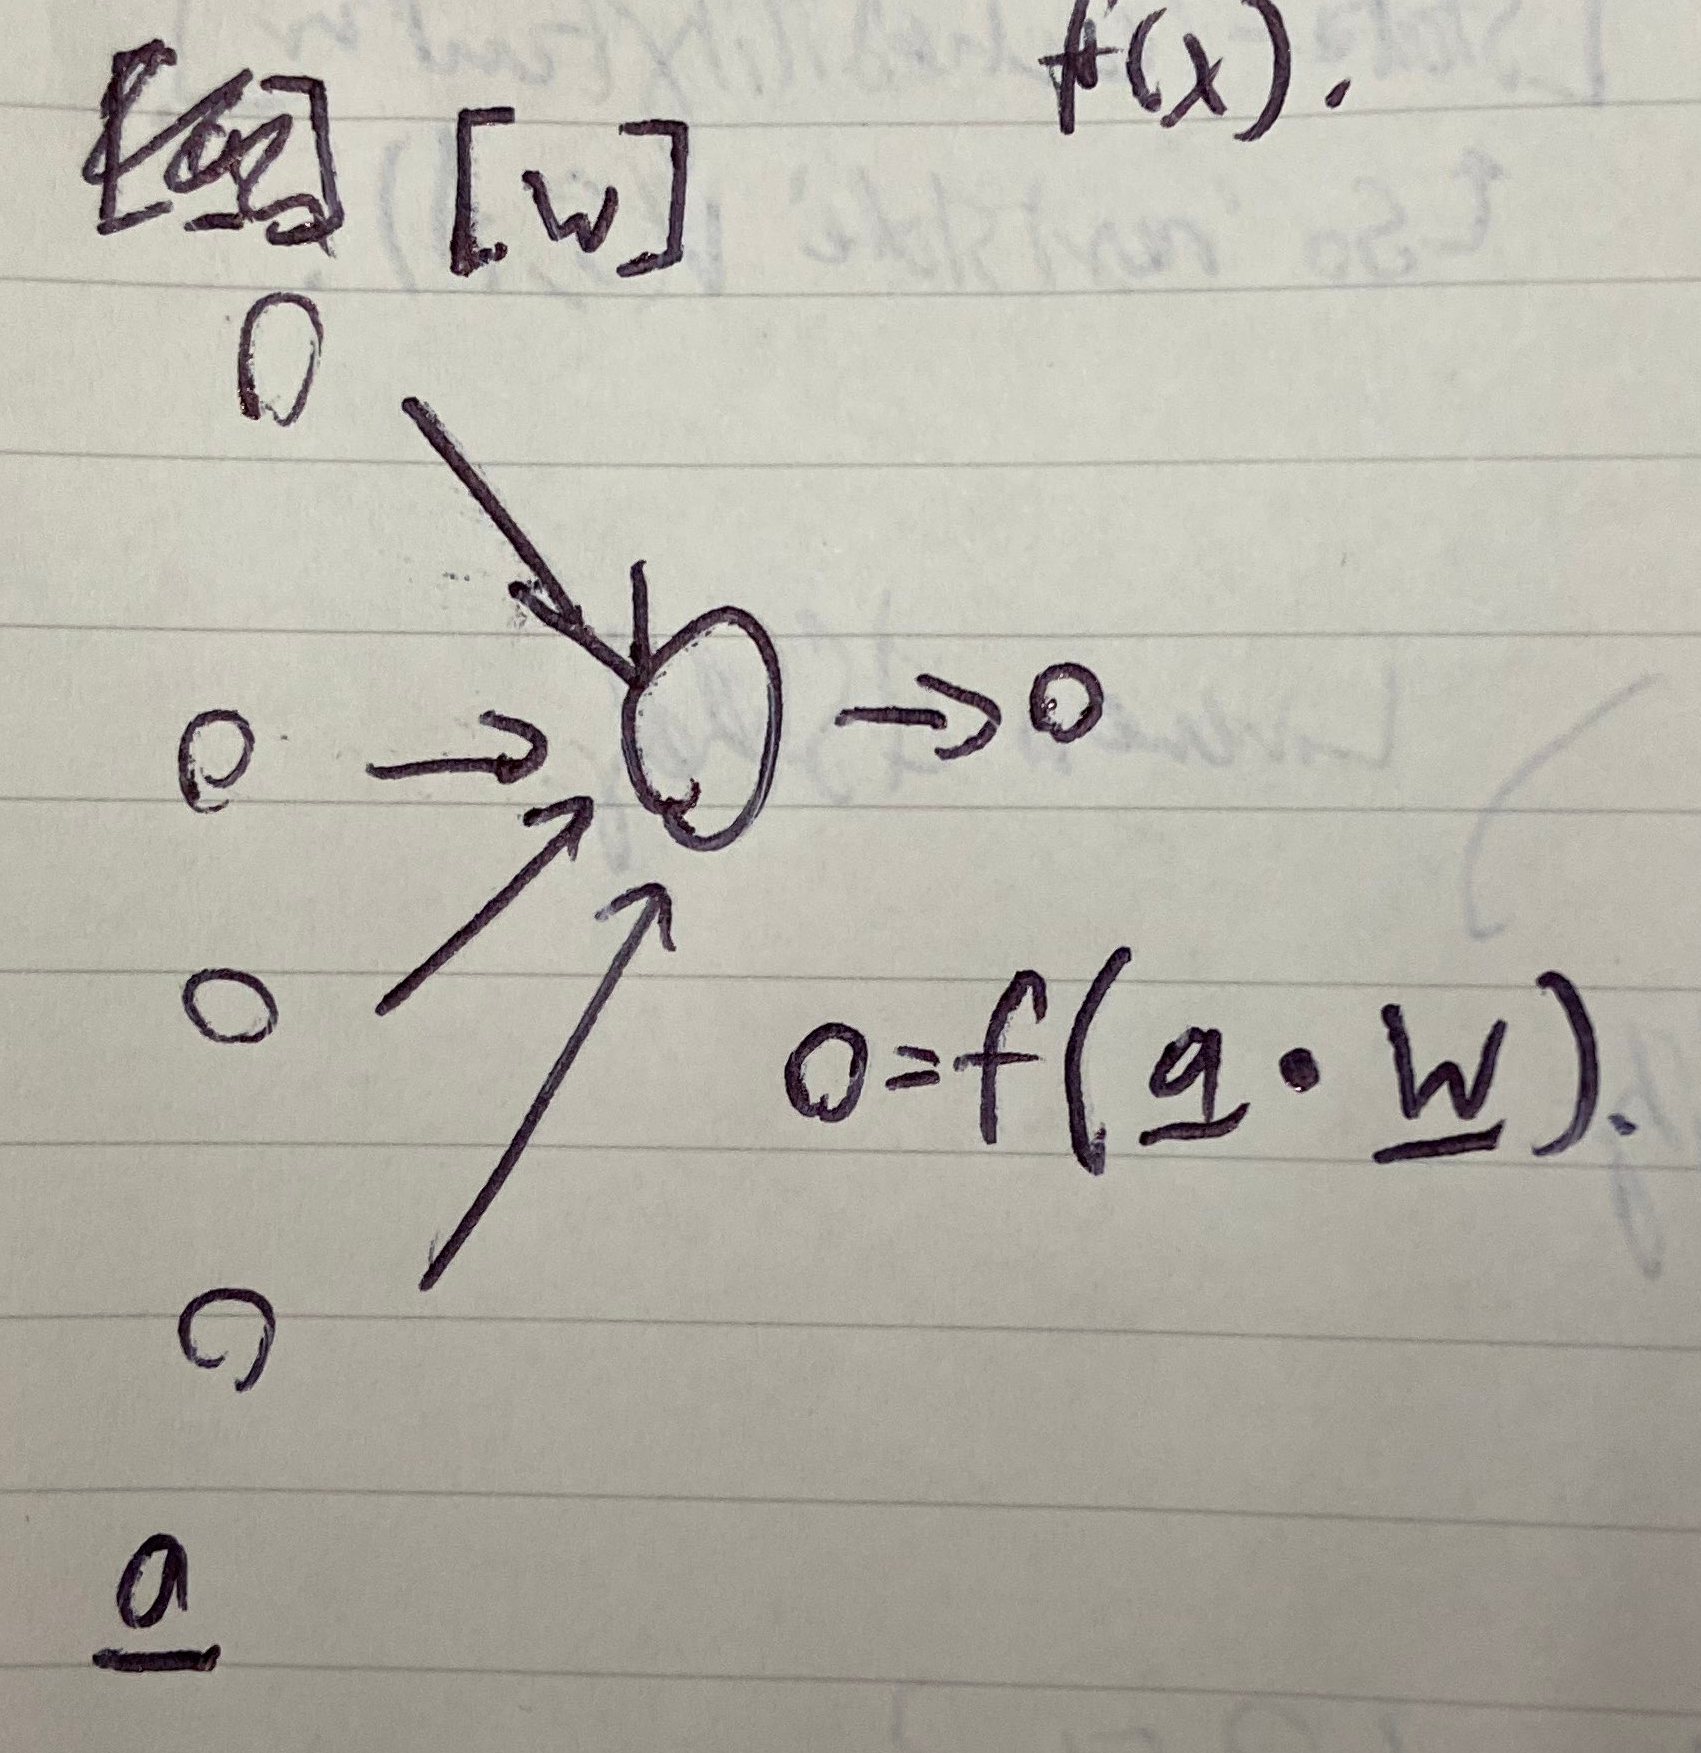
\includegraphics{diagrams/nns/single-neuron-draft}}
	\caption[Operation of a single neuron.]{A single neuron in a \gls{acr:nn} takes a weighted sum over its vector of inputs $\mathbf{a}$ (according to $\mathbf{w}$) and its own bias $b$, and produces an output using some non-linear $f$. $\mathbf{w}$ and $b$ are trainable per neuron. ?? Note, diagram misses out bias...}\label{fig:single-neuron}
\end{marginfigure}

\begin{figure}
	\centering
	\resizebox{0.9\linewidth}{!}{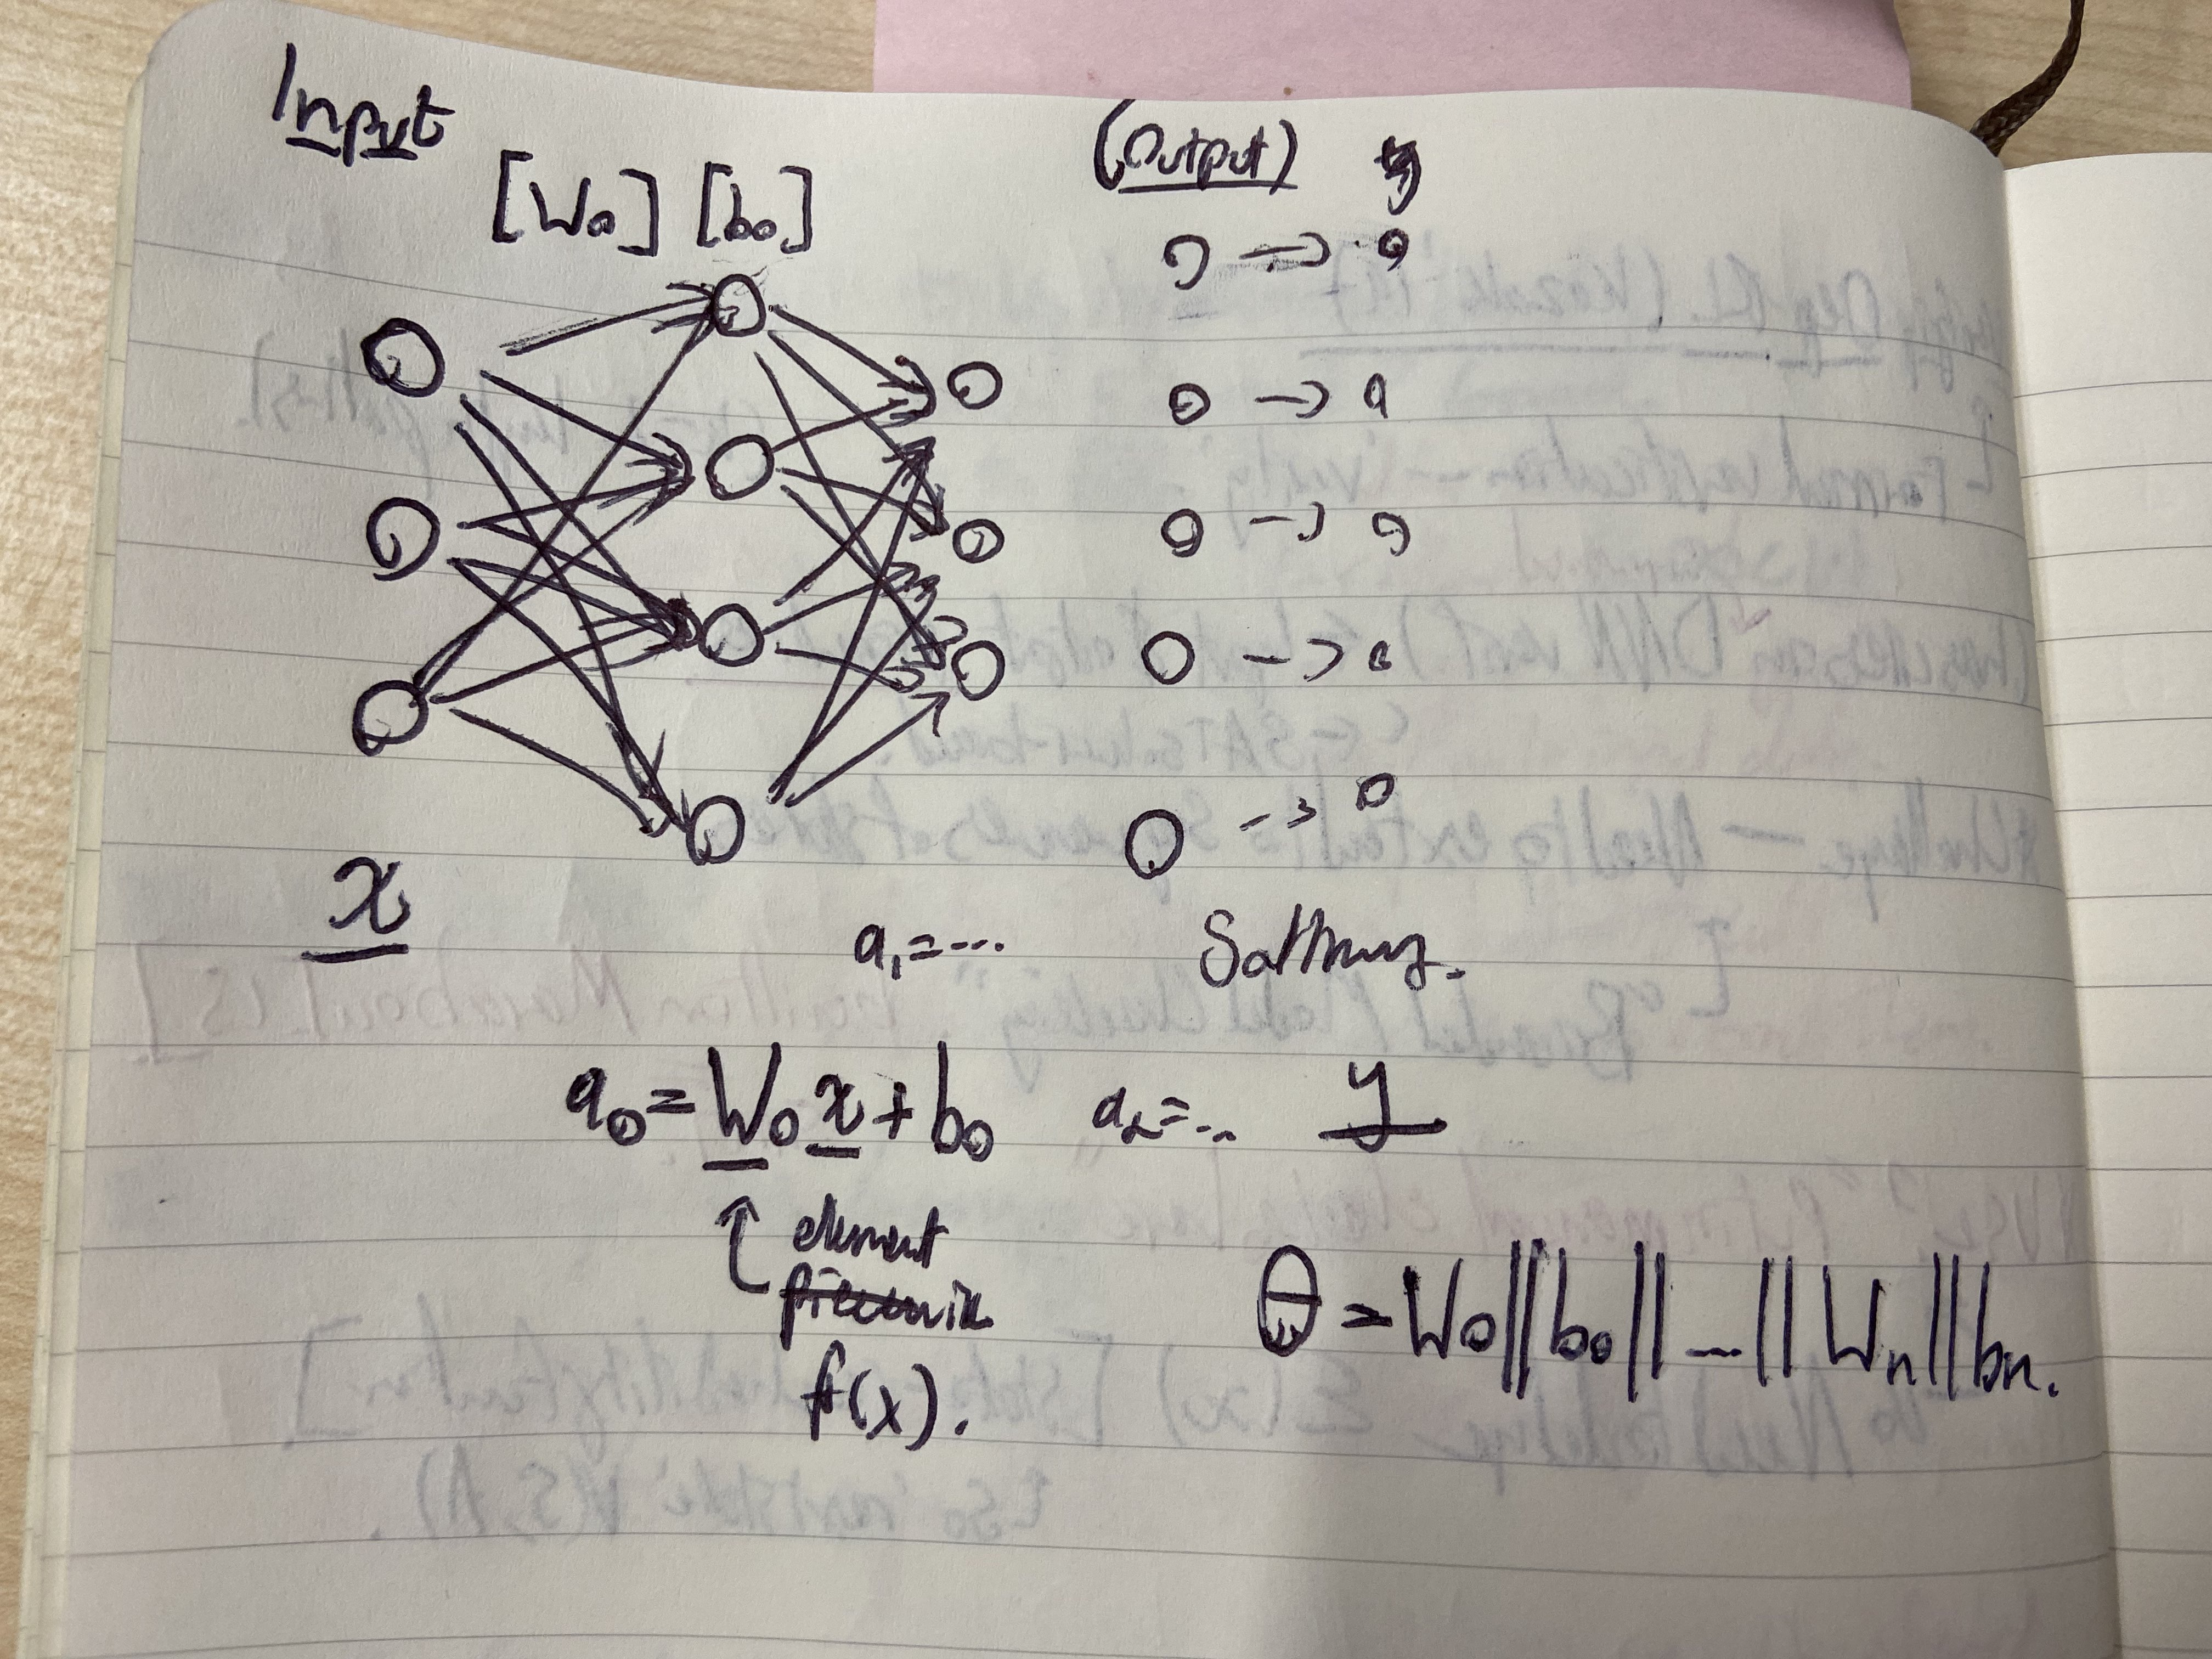
\includegraphics{diagrams/nns/fcnn-draft}}
	\caption[An example fully-connected neural network.]{\glspl{acr:nn} arrange neurons into layers, which allows each layer to be expressed as an affine transformation (i.e., $\mathbf{W}_i\mathbf{a}_{i-1} + \mathbf{b}_i$) followed by an elementwise non-linear operation. By doing so, they can take advantage of commodity \glspl{acr:gpu} (which excel at linear algebra) or more specialised \glspl{acr:tpu}.}\label{fig:fcnn}
\end{figure}

\paragraph{Convolutional networks}

\paragraph{Graph convolution}
?? GNNs -- GCN, Edge-GNNs~\parencite{Mirhoseini2021}

?? graph convolution~\parencite{DBLP:conf/iclr/KipfW17}

\paragraph{Recurrent networks}
\gls{acr:lstm}~\parencite{DBLP:journals/neco/HochreiterS97}

\section{Learning an approximation}\label{sec:learning-an-approximation}%
Having introduced function approximation schemes of relevance to this thesis (and the most prominent in \gls{acr:ddn} at present), we now turn our attention to how these approximators are trained in practice.
Due to its relevance in \gls{acr:dnn} and \gls{acr:drl}, this comprises a brief discussion of gradient descent techniques and stochastic optimisers, followed by a more in-depth introduction to and overview of the field of \gls{acr:rl}.
Tying these back to the realities of \gls{acr:ddn}, many of these techniques and advances are likely feasible in a \gls{acr:pdp} context with small datasets and no minibatches, such as the variants of \gls{acr:sgd}, but their use is left to future work.

We can begin by assuming that our approximate function is backed by some \emph{parameter vector} $\wvec{}$, such that $\hat{\symbfit{y}} = f{\left(\symbfit{x}~|~\wvec{}\right)}$---an input vector $\symbfit{x}$ produces some output $\hat{\symbfit{y}}$, and ideally after training $\hat{\symbfit{y}}\eqsim\symbfit{y}$ across all input $\symbfit{x}$.
For all intents and purposes, we can understand $\wvec{}$ as a large block of real numbers residing in \gls{acr:ram}, and that we update this block over time.
We may not have access to a ground-truth $\symbfit{y}$ (i.e., in the \gls{acr:rl} case), but we generally assume that there does exist a best-fitting or optimal output.
In case we do, however, we may refer to the complete set of training inputs and ground-truth outputs as $\symbfit{X}$.
Crucially, we require that $f$ is differentiable with respect to $\wvec{}$: if we define some scalar performance metric $J$ which assesses the quality of an output $\hat{\symbfit{y}}$, then $\nabla_{\wvec{}}{J}$ offers a direction in $\wvec{}$.\sidenote{In the definition of $J$, we naturally expand occurrences of $\hat{\symbfit{y}}$ in terms of $f$, and thus $\wvec{}$. Additionally, $J$ may be defined over any subset (or all) of the training set $\symbfit{X}$.}
This output gradient is simply a vector, which represents the direction in parameter-space which  would have the largest \emph{increase} in the value of $J$ if followed.
The approaches presented in \cref{sec:function-approximation} provide just this.

\subsection{Gradient descent}
%Supervised and unsupervised methods alike typically offer clear ways to map from the model parameters we have at this moment, and our performance on a training dataset, into a \emph{loss function}.
Most supervised \gls{acr:ml} problems are defined in terms of a \emph{loss function} $L$, such that differences between our output $\hat{\symbfit{y}}$ and $\symbfit{y}$ values are penalised.
Some examples in use today include the mean absolute and mean squared errors ($L_1$ and $L_2$ loss) in regression tasks, or (categorical) cross-entropy loss in classification.
Naturally, these are differentiable, but as we aim to \emph{minimise} loss we then \emph{subtract} the gradient from $\wvec{}$; this concept underlies \emph{gradient descent}.
Gradient descent is the iterative process of optimising our parameter vector $\wvec{}$, using all input data and labels $\symbfit{X}$ at each iteration:
\begin{equation}
	\wvec{t+1} = \wvec{t} - \alpha\nabla_{\wvec{t}}{L\left(\symbfit{X}~|~\wvec{t}\right)}
\end{equation}
Every iteration, we move the parameter vector a small step in the direction which would optimise its overall performance; this is the learning rate hyperparameter $\alpha\in\left(0,1\right)$.
However, re-evaluating the loss function over all input data becomes intractable in the case that either the function is expensive to compute on a moderately-sized dataset, or the dataset itself is monstrously large.
Both are often the case in \gls{acr:dnn} training.
It is for this reason that \gls{acr:sgd} and related algorithms are typically employed in \gls{acr:ml} model training, particularly for \glspl{acr:dnn}.
\gls{acr:sgd} modifies the above such that individual, randomly chosen samples (or larger minibatches) are used as the input for the loss function rather than the entire dataset.
This only approximates the loss gradient at $\wvec{}$ on the input data, but in practice this is key for the training of modern \gls{acr:ml} techniques---$\alpha$ may be reduced over time and the dataset reshuffled as necessary until convergence.

While \gls{acr:sgd} provides the theoretical underpinning for more efficient \gls{acr:ml} training, in practice the difficulty of choosing $\alpha$ with regard to different parameter sensitivity has led to more adaptive methods.
These also introduce the notion of per-parameter learning rates.
\emph{AdaGrad}~\parencite{DBLP:journals/jmlr/DuchiHS11} gives each parameter its own learning rate $\alpha$, divided by the square root of the sum of squared gradient values (i.e., large derivatives in a parameter lead to a greater reduction in learning rate).
\emph{RMSProp}~\parencite{rmsprop} converts this accumulation into an exponentially-weighted moving average, better handling the non-convex loss behaviour seen in \gls{acr:dnn} training.
\emph{Adam}~\parencite{DBLP:journals/corr/KingmaB14} includes momentum terms (to carry a general direction in gradient across several steps) and additional bias correction, giving advantages in the early stages of training.

It should be noted that the above discussion is a very cursory treatment of the subject, primarily intended to contrast the in-depth discussion of \gls{acr:rl} methods in the remainder of the section.
Similarly, learning-centric modifications to loss functions such as regularisation terms or function-specific regularisation strategies (to mitigate overfitting) are also out of scope.
For more details, readers should refer to more specialised texts such as \Textcite{DBLP:journals/siamrev/BottouCN18, DBLP:books/daglib/0040158}.

\begin{marginfigure}
	\centering
	\resizebox{0.9\linewidth}{!}{\centering
\begin{tikzpicture}
	\node[circle, draw] (meadow) {};

	\node[circle, draw, fill=example-swamp] (swamp) at ($(meadow) + (-1, -1.5)$) {};
	\node[circle, draw, fill=example-steppe] (steppe) at ($(meadow) + (+1, -1.5)$) {};
	
	\node[circle, draw, fill=example-forest] (forest) at ($(swamp) + (+0, -1.5)$) {};
	\node[circle, draw, fill=example-desert] (desert) at ($(steppe) + (+0, -1.5)$) {};

	\node[circle, draw, double, fill=example-castle] (castle) at ($(forest) + (+1, -1.5)$) {};
	
	% \node (agent) at ($(2, 0) + (state)$) {Agent};
	% \node[below of=agent] (action) {Action $A$};
	
	% \node[right of=state'] {$+ R$};
	
	\draw[->] ($(meadow) + (0, 1)$) -- (meadow);

	\draw[->, dashed] (meadow) -- (swamp) node[midway, left] {\small \textsc{Sw}};
	\draw[->, dashed] (meadow) -- (steppe) node[midway, right] {\small \textsc{Se}};

	\path[->, dashed] (swamp) edge[bend right=45] node [left] {\small \textsc{Sw}} (forest);
	\path[->, dashed] (swamp) edge[bend left=45] node [right] {\small \textsc{Se}} (forest);

	\path[->, dashed] (steppe) edge[bend right=45] node [left] {\small \textsc{Sw}} (desert);
	\path[->, dashed] (steppe) edge[bend left=45] node [right] {\small \textsc{Se}} (desert);

	\draw[->, dashed] (desert) -- (castle) node[midway, right] {\small \textsc{Sw}};
	\draw[->, dashed] (forest) -- (castle) node[midway, left] {\small \textsc{Se}};

	\node[above left of=swamp, align = center] {{\bfseries\color{example-swamp}Swamp}\\$R$ = \num{-1}};
	\node[below left of=forest, align = center] {{\bfseries\color{example-forest}Forest}\\$R$ = 10};
	\node[above right of=steppe, align = center] {{\bfseries\color{example-steppe}Steppe}\\$R$ = 1};
	\node[below right of=desert, align = center] {{\bfseries\color{example-desert}Desert}\\$R$ = \num{-10}};
	\node[below of=castle, align = center] {{\bfseries\color{example-castle}Castle}\\$R$ = 5};
	
	% \draw[dotted, ->, bend left = 30] (state) -- (agent);
	% \draw[->] (agent) -- (action);
	% \draw[dotted, ->] (action) -- (state);
\end{tikzpicture}}
	\caption[A motivating example for MDPs in handling delayed rewards.]{A toy example showing how the \emph{delayed rewards} which an \gls{acr:rl} agent learns to maximise. Consider a traveller journeying towards a castle in the south, with $R$ being some aggregate of food, water and rest. Learning only to optimise immediate rewards attached to actions would lead our traveller to choose an overall worse path---going thirsty in the desert!}\label{fig:toy-rl-motiv}
\end{marginfigure}

\subsection{Reinforcement learning}
When we aim to optimise for decisions and estimations in classification, clustering, and regression, it suffices to apply gradient descent and similar optimisers to minimise this loss function alone.
How might things differ when we want to design some \emph{agent}---an actor who sees and acts on a system for many timesteps---to interact with the world?
Consider a toy example in \cref{fig:toy-rl-motiv}: an oracle with global knowledge knows that a hypothetical traveller would best be served by going through the swamp, even if it appears the worse of two choices.
Yet if we applied simple input classification to choose our path at each turn, we would always act poorly without some way of propagating knowledge of later choices.
It becomes more complex to collect training data once we realise that our actions move the world forward and change it (thus we may not be able to rewind a simulation to explore alternative choices), and that we might need to explore apparently suboptimal choices for some time to be better off in aggregate.

\glsxtrfull{acr:rl} algorithms are methods of training such an agent to choose an optimal sequence of actions in pursuit of a given task~\parencite{RL2E}, and neatly encode these training- and run-time notions of \emph{exploration} and \emph{exploitation}.
An agent is typically defined by its \emph{policy} $\pi$, which chooses an action in response to an input state.
These powerful techniques effectively use a \emph{reward} metric to learn a state-action mapping without any explicit model of the system they're learning to control---even when reward signals are sparse or come with some delay after an initial choice.

To achieve the goals described above, we first make the assumption that the task we're attempting to solve is structured as an \gls{acr:mdp}.
In an \gls{acr:mdp}, we break the world or target problem down into a set of \emph{states} ($\mathcal{S}$), \emph{actions} ($\mathcal{A}$), and \emph{reward measurements} ($\mathbb{R}$).
To relate this to computer networks, an example state space would be a vector of buffer occupancies in a switch, an action space would be the priority to assign some new flow which has arrived, and the reward might be the proportion of finished flows which achieved comfortably low \glspl{acr:fct}.
We then consider our sequence of interactions in discrete \emph{timesteps}---at the present time $t$, an agent observes $s_t \in \mathcal{S}$, chooses some $a_t \in \mathcal{A}$, and then observes their change in the world as a new state $s_{t+1} \in \mathcal{S}$ and a reward measure $r_{t+1} \in \mathbb{R}$.
As required, we can qualify these further, e.g., the set of actions we can take from a state $s$ may be limited to $A_s \subseteq \mathcal{A}$.
Acting optimally then consists of maximising the sum of rewards over some time horizon.
This is captured up to an infinite horizon by the concept of the \emph{expected discounted return}:
\begin{equation}
	\mathbb{E}\left[\sum_{t=0}^{\infty}\gamma^{t}R_t\right]
\end{equation}
where the \emph{discount} $\gamma \in \left[0,1\right]$ controls how ``forward-planning'' an agent may be\sidenote{Setting $\gamma=0$ defines a `myopic' agent, where no intermediate loss of reward is allowed. Choosing $\gamma=1$ will prioritise future rewards, with no concern over how long it may take to achieve those rewards. This hyperparameter features in many \gls{acr:rl} algorithms; in practice, we choose values closer to \num{1}.}, always choosing $a_t \sim \pi\left(a_t~|~s_t,\wvec{t}\right)$.
While dense, this formalism essentially captures and describes the performance of our agent over all possible run-lengths from all starting states (i.e., over all \emph{episodes}), and in general this is what \gls{acr:rl} algorithms are designed to maximise.

\glspl{acr:mdp} assume that there are stationary, well-defined (though stochastic) transitions between these states.
For any $s, s' \in \mathcal{S}, a \in A_s$, an \gls{acr:mdp} is defined by a state transition function, $\operatorname{P_a}\left(s,s'\right)$ which returns the probability that we will land in $s'$ after taking action $a$ in state $s$, and a function returning the \emph{expected reward} $\operatorname{R_a}\left(s,s'\right)$ for each valid transition.
If we have all this information, then we can apply the Bellman equation~\parencite{10.2307/24900506}, a dynamic programming algorithm, to solve for an optimal policy.
This allows us to assign a \emph{value} $v_\pi{\left(s\right)}$ to each state (the expected return over all choices in the current state), and $q_\pi{\left(s,a\right)}$ to each action, and then choose maximal-value actions at each timestep.
In real-world scenarios however, we usually lack this knowledge; this either requires involved modelling, or is rendered intractable by a continuous or combinatorially large state space.

Like most \gls{acr:ml} methods, modern \gls{acr:rl} algorithms use gradient information to update the parameters used to approximate a function.
How \gls{acr:rl} differs is that it aims to learn an optimal policy without any knowledge of the \gls{acr:mdp} apart from its state and action space---\emph{model-free}.
Knowledge of the \emph{trajectories} followed by agents (i.e., state-action-reward tuples at all timesteps) is then used to compute target values and adjustments for the parameter set $\wvec{}$ for any function approximator.
By requiring that our policy approximation $\pi\left(a~|~s, \wvec{} \right)$ is differentiable, \gls{acr:rl} works in tandem with any of the function approximation approaches described in \cref{sec:function-approximation}.\sidenote{Note the policy $\pi$ does not require any knowledge of rewards, except when training. This allows for \gls{acr:rl} agents to be trained using simulated systems or data, and then deployed in an environment where they cannot access this knowledge due to sampling cost. If these measures are present in deployment, then \gls{acr:rl} can learn online.}

%\gls{acr:rl} works in tandem with other mathematical training approaches: the key insight is that the structure of an MDP allows external information and model(-free) observation to strengthen or weaken different function responses.

\subsection{Demonstrating RL: Sarsa}\label{sec:demo-rl-sarsa}
While many \gls{acr:rl} algorithms have been developed (each of which making quite different choices on how to apply trajectory data), it is likely most helpful to start with a concrete point in the design space \emph{before} listing their full variety.
Doubly so here, as this particular algorithm---single-step, semi-gradient Sarsa~\parencite[pp. \numrange{217}{221}]{RL2E}---underpins \cref{chap:ddos-rl,chap:in-net-rl}.
The Sarsa algorithm considers only one transition at a time: a pair of states $s_t,s_{t+1}$, their accompanying actions $a_t,a_{t+1}$, and the reward $r_{t+1}$ accompanying $s_{t+1}$.
This is why it is defined as \emph{single-step}, and as such it does not require a completed trajectory for learning.

%Assume first that $\wvec{}$ is a large block of real numbers residing in \gls{acr:ram}, and that we update this block through time.
As Sarsa is a \emph{value-based} method, an agent operates by defining an approximate \emph{value} function $\acval{s}{a}{\wvec{}}$ to each action $a$ it can take from $s$, typically choosing the action with the highest value.
Note that $\acvalblank$ is completely arbitrary, and may be any differentiable approximator.
We can then update $\wvec{}$ over time as follows:
\begin{subequations}
	\begin{gather}
		\delta_t = r_{t+1} + \gamma \acval{s_{t+1}}{a_{t+1}}{\wvec{t}} - \acval{s_t}{a_t}{\wvec{t}},\label{eqn:sg-sarsa-td}\\
		\wvec{t+1} = \wvec{t} + \alpha \delta_t \nabla{\acval{s_t}{a_t}{\wvec{t}}},\label{eqn:sg-sarsa-update}
	\end{gather}%
	\label{eqn:sg-sarsa}%
	where $\delta_t$ is known as the \gls{acr:td} error. $\alpha\in\left(0,1\right)$ defines the learning rate (governing the policy stability), with $\gamma$ defined as in the \gls{acr:mdp} formulation.
\end{subequations}

In essence, at each timestep the policy parameters ($\wvec{}$) are increased along the gradient ($\nabla{\acvalblank}$) using a fixed learning rate ($\alpha$) and a computed adjustment ($\delta_t$).
This adjustment is equal to the difference between the chosen action $a$'s value in state $s$ and the reward received ($r_{t+1} - \acval{s_t}{a_t}{\wvec{}}$), plus some part of the \emph{next} action's value ($\gamma\acval{s_{t+1}}{a_{t+1}}{\wvec{}}$).
Naturally, as state transitions are visited and revisited during training, the value of later choices can propagate down the tree of states, as shown by \cref{fig:sarsa-intuition}.
To see how this combines with a simple linear function approximation, consider \cref{fig:sarsa-tilecode,fig:sarsa-tilecode-update}.

\begin{marginfigure}
	\resizebox{0.9\linewidth}{!}{\centering
\begin{tikzpicture}
	\node[circle, draw] (state) {};

	\node[circle, draw] (state') at ($(state) + (-0.5, -1)$) {};
	\node[circle, draw, dashed] (stateg') at ($(state') + (0.5, 0)$) {};
	\node[circle, draw, dashed] (stategg') at ($(stateg') + (0.5, 0)$) {};

	\node[circle, draw, dashed] (state'') at ($(state') + (-0.5, -1)$) {};
	\node[circle, draw, dashed] (stateg'') at ($(state'') + (0.5, 0)$) {};
	\node[circle, draw] (stategg'') at ($(stateg'') + (0.5, 0)$) {};

	\draw[->] (state) -- (state');
	\draw[->, dashed] (state) -- (stateg');
	\draw[->, dashed] (state) -- (stategg');

	\draw[->, dashed] (state') -- (state'');
	\draw[->, dashed] (state') -- (stateg'');
	\draw[->] (state') -- (stategg'');

	\path[->, color=uofgrust] (stategg'') edge[bend right=45] node [right] {\tiny $\gamma\acvalblank$} (state');
	\path[->, color=uofgrust] (state') edge[bend left=45] node [left] {\tiny $\gamma^2\acvalblank$} (state);
\end{tikzpicture}}
	\caption[An illustration of how value adjustments in single-step RL propagate backwards through a state trajectory.]{A simplified view of how action values propagate back through visited states: because a state's value includes some portion $\gamma$ of its children's values, at convergence it includes $\gamma^2$ of its grandchildren, and so on. A limitation of the single-step family is that they must visit the same transitions several times for earlier states to learn about their successors.}\label{fig:sarsa-intuition}
\end{marginfigure}

\begin{figure}
	\centering
	\begin{subfigure}{0.6\linewidth}
		\resizebox{\linewidth}{!}{\begin{tikzpicture}
	\node at (0,0.3){$s = \begin{pmatrix}
			0.7 \\
			0.3
		\end{pmatrix}$};
	\node at (0,-1) {$\symbfit{x}(s,\cdot) = \begin{Bmatrix}
			T_{1,9}, \\
			T_{2,5}, \\
			T_{\mathit{bias}}
		\end{Bmatrix}$};
	
	\node at (2.5,-0.5) {
		\begin{tikzpicture}
			\draw[step=0.5cm,color=uofgcobalt,opacity=0.7,shift={(0,0)},label=above:{Tiling 0}] (-0.5,-0.5) grid (1,1);
			\fill[uofgcobalt,opacity=0.5] (0.5,-0.5) rectangle (1,0);
			\node[color=uofgcobalt] at (0,1.1) {\footnotesize Tiling 1};
			
			\draw[step=0.5cm,color=uofgpumpkin,opacity=0.9,shift={(0.25,-0.25)},label=above:{Tiling 1}] (-0.5,-0.5) grid (1,1);
			\fill[uofgpumpkin,opacity=0.5,shift={(0.25,-0.25)}] (0,0) rectangle (0.5,0.5);
			\node[color=uofgpumpkin!50!uofgrust] at (0.25,-0.95) {\footnotesize Tiling 2};
			
			\node[circle, black, draw,
			fill, radius=0.5pt, inner sep=0pt,minimum size=1.5pt, label=above:{$s$}] at (0.625,-0.125) {};
			%			\filldraw (0.625,-0.125) circle[radius=1.5pt,label=above:{$s$}];
			
			\draw[->] (-0.25,-0.5)--(-0.25,0.85);
			\draw[->] (-0.25,-0.5)--(1.1,-0.5);
			
			\node at (1,-0.7) {\footnotesize 1};
			\node at (-0.4,0.75) {\footnotesize 1};
			\node at (-0.35,-0.6) {\footnotesize 0};
		\end{tikzpicture}
	};
	
\end{tikzpicture}}
		\caption{Tile Coding\label{fig:tilecode-code}}
	\end{subfigure}

	\begin{subfigure}{0.6\linewidth}
		\resizebox{\linewidth}{!}{\begin{tikzpicture}
	% Top half
	\def\topacs{
		{-0.3,-0.5,-0.1,0.8},
		{0.1,0.1,-0.2,0.3},
		{0.3,0.4,0.2,-0.4}%
	}
	
	\foreach \line [count=\y] in \topacs {
		\foreach \pix [count=\x] in \line {
			\ifthenelse{\lengthtest{\pix pt < 0 pt}}{
				\pgfmathtruncatemacro\lambda{(\pix+1)*100}
				\draw[shift={(-0.7,0)},fill=midac!\lambda!lowac] (0.7*\x,-0.35*\y) rectangle +(0.7,0.35);
			}{
				\pgfmathtruncatemacro\lambda{\pix*100}
				\draw[shift={(-0.7,0)},fill=highac!\lambda!midac] (0.7*\x,-0.35*\y) rectangle +(0.7,0.35);
			}
			\node[shift={(-0.35,0.175)}] at (0.7*\x,-0.35*\y) {\footnotesize \pix};
		}
	}
	
	\draw[xstep=0.7cm,ystep=0.35cm,shift={(0,0)}] (0,-1.06) grid (2.8,0);
	\node[label=left:{$T_{1,9}$},shift={(0,-0.125)}] at (0,0) {}; 
	\node[label=left:{$T_{2,5}$},shift={(0,-0.125)}] at (0,-0.375) {}; 
	\node[label=left:{$T_{\mathit{bias}}$},shift={(0,-0.125)}] at (0,-0.75) {};
	
	% bottom half
	\def\botacs{
		{0.1,0.0,-0.1,0.7}%
	}
	
	\foreach \line [count=\y] in \botacs {
		\foreach \pix [count=\x] in \line {
			\ifthenelse{\lengthtest{\pix pt < 0 pt}}{
				\pgfmathtruncatemacro\lambda{(\pix+1)*100}
				\draw[shift={(-0.7,-1.275)},fill=midac!\lambda!lowac] (0.7*\x,-0.35*\y) rectangle +(0.7,0.35);
			}{
				\pgfmathtruncatemacro\lambda{\pix*100}
				\draw[shift={(-0.7,-1.275)},fill=highac!\lambda!midac] (0.7*\x,-0.35*\y) rectangle +(0.7,0.35);
			}
			\node[shift={(-0.35,-1.1)}] at (0.7*\x,-0.35*\y) {\footnotesize \pix};
		}
	}
	
	\draw[xstep=0.7cm,ystep=0.35cm,shift={(0,-1.275)}] (0,-0.35) grid (2.8,0);
	\node[label=left:{$\mathit{Total}$},shift={(0,-0.175)}] at (0,-1.275) {};
	
	\draw [->] (2.45, -1.9) -- (2.45, -1.65);
\end{tikzpicture}}
		\caption{\centering Value Estimation and Action Selection\label{fig:tilecode-select}}
	\end{subfigure}
	
	\caption[An end-to-end example of Sarsa selecting an action using a tile-coded policy.]{
		An example of tile coding for 2-dimensional state and 4 actions, using 2 tilings, 3 tiles per dimension, and a bias tile.
		All components of $s$ are clamped to $[0,1]$.
		For simplicity, I denote $\symbfit{x}(s,\cdot)$ as a list of indices and represent the values of all actions at each tile with a vector.
		(a) The state $s$ activates the bias tile and exactly one tile in each tiling.
		(b) The action values of active tiles are summed to produce the current value estimate for each action available in $s$---for this state, local knowledge ensures that action 4 is chosen by the greedy policy despite typically being a poor choice elsewhere.
		\label{fig:sarsa-tilecode}
	}
\resizebox{0.6\linewidth}{!}{\begin{tikzpicture}		
	% Top half
	\def\startacs{
		{0.8},
		{0.3},
		{-0.4}%
	}
	
	\foreach \line [count=\y] in \startacs {
		\foreach \pix [count=\x] in \line {
			\ifthenelse{\lengthtest{\pix pt < 0 pt}}{
				\pgfmathtruncatemacro\lambda{(\pix+1)*100}
				\draw[shift={(-0.7,0)},fill=midac!\lambda!lowac] (0.7*\x,-0.35*\y) rectangle +(0.7,0.35);
			}{
				\pgfmathtruncatemacro\lambda{\pix*100}
				\draw[shift={(-0.7,0)},fill=highac!\lambda!midac] (0.7*\x,-0.35*\y) rectangle +(0.7,0.35);
			}
			\node[shift={(-0.35,0.175)}] at (0.7*\x,-0.35*\y) {\footnotesize \pix};
		}
	}
	
	\draw[xstep=0.7cm,ystep=0.35cm,shift={(0,0)}] (0,-1.06) grid (0.7,0);
	\node[label=left:{$T_{1,9}$},shift={(0,-0.125)}] at (0,0) {}; 
	\node[label=left:{$T_{2,5}$},shift={(0,-0.125)}] at (0,-0.375) {}; 
	\node[label=left:{$T_{\mathit{bias}}$},shift={(0,-0.125)}] at (0,-0.75) {};
	\node[label=below:{\footnotesize Action 4},shift={(0.35,-0.125)}] at (0,-0.75) {};
	\node[label=above:{\footnotesize $\wvec{t}$},shift={(0.35,-0.125)}] at (0,0) {};
	
	\def\finalacs{
		{0.7},
		{0.2},
		{-0.5}%
	}
	
	\foreach \line [count=\y] in \finalacs {
		\foreach \pix [count=\x] in \line {
			\ifthenelse{\lengthtest{\pix pt < 0 pt}}{
				\pgfmathtruncatemacro\lambda{(\pix+1)*100}
				\draw[shift={(2-0.7,0)},fill=midac!\lambda!lowac] (0.7*\x,-0.35*\y) rectangle +(0.7,0.35);
			}{
				\pgfmathtruncatemacro\lambda{\pix*100}
				\draw[shift={(2-0.7,0)},fill=highac!\lambda!midac] (0.7*\x,-0.35*\y) rectangle +(0.7,0.35);
			}
			\node[shift={(2-0.35,0.175)}] at (0.7*\x,-0.35*\y) {\footnotesize \pix};
		}
	}
	
	\draw[xstep=0.7cm,ystep=0.35cm,shift={(2,0)}] (0,-1.06) grid +(0.7,1.06);
	\node[label=below:{\footnotesize Action 4},shift={(2.35,-0.125)}] at (0,-0.75) {};
	\node[label=above:{\footnotesize $\wvec{t+1}$},shift={(0.35,-0.125)}] at (2,0) {};
	
	\draw[->] (0.9,-0.5) -- node[above] {$+ \alpha \delta_t$} (1.8,-0.5);
\end{tikzpicture}}
\caption[An end-to-end example of Sarsa updating the values for a chosen action using a tile-coded policy.]{
	The update step for \cref{fig:sarsa-tilecode}, given an observed \gls{acr:td} error $\delta_t=-0.2$ (indicating a lower observed reward than the expected long-term value of \num{0.7}) and $\alpha=0.5$.
	Action 4's value is thus reduced in the tiles associated with state $s$, but remains the most likely choice; the negative $\delta_t$ may have arisen from noise in the reward signal.
	For illustrative purposes, I choose an unrealistically high $\alpha$ (typically, $\alpha\le0.05$ is a more reasonable choice).
	\label{fig:sarsa-tilecode-update}
}
\end{figure}

%\begin{figure}
%	\centering
%	\resizebox{0.6\linewidth}{!}{\begin{tikzpicture}		
	% Top half
	\def\startacs{
		{0.8},
		{0.3},
		{-0.4}%
	}
	
	\foreach \line [count=\y] in \startacs {
		\foreach \pix [count=\x] in \line {
			\ifthenelse{\lengthtest{\pix pt < 0 pt}}{
				\pgfmathtruncatemacro\lambda{(\pix+1)*100}
				\draw[shift={(-0.7,0)},fill=midac!\lambda!lowac] (0.7*\x,-0.35*\y) rectangle +(0.7,0.35);
			}{
				\pgfmathtruncatemacro\lambda{\pix*100}
				\draw[shift={(-0.7,0)},fill=highac!\lambda!midac] (0.7*\x,-0.35*\y) rectangle +(0.7,0.35);
			}
			\node[shift={(-0.35,0.175)}] at (0.7*\x,-0.35*\y) {\footnotesize \pix};
		}
	}
	
	\draw[xstep=0.7cm,ystep=0.35cm,shift={(0,0)}] (0,-1.06) grid (0.7,0);
	\node[label=left:{$T_{1,9}$},shift={(0,-0.125)}] at (0,0) {}; 
	\node[label=left:{$T_{2,5}$},shift={(0,-0.125)}] at (0,-0.375) {}; 
	\node[label=left:{$T_{\mathit{bias}}$},shift={(0,-0.125)}] at (0,-0.75) {};
	\node[label=below:{\footnotesize Action 4},shift={(0.35,-0.125)}] at (0,-0.75) {};
	\node[label=above:{\footnotesize $\wvec{t}$},shift={(0.35,-0.125)}] at (0,0) {};
	
	\def\finalacs{
		{0.7},
		{0.2},
		{-0.5}%
	}
	
	\foreach \line [count=\y] in \finalacs {
		\foreach \pix [count=\x] in \line {
			\ifthenelse{\lengthtest{\pix pt < 0 pt}}{
				\pgfmathtruncatemacro\lambda{(\pix+1)*100}
				\draw[shift={(2-0.7,0)},fill=midac!\lambda!lowac] (0.7*\x,-0.35*\y) rectangle +(0.7,0.35);
			}{
				\pgfmathtruncatemacro\lambda{\pix*100}
				\draw[shift={(2-0.7,0)},fill=highac!\lambda!midac] (0.7*\x,-0.35*\y) rectangle +(0.7,0.35);
			}
			\node[shift={(2-0.35,0.175)}] at (0.7*\x,-0.35*\y) {\footnotesize \pix};
		}
	}
	
	\draw[xstep=0.7cm,ystep=0.35cm,shift={(2,0)}] (0,-1.06) grid +(0.7,1.06);
	\node[label=below:{\footnotesize Action 4},shift={(2.35,-0.125)}] at (0,-0.75) {};
	\node[label=above:{\footnotesize $\wvec{t+1}$},shift={(0.35,-0.125)}] at (2,0) {};
	
	\draw[->] (0.9,-0.5) -- node[above] {$+ \alpha \delta_t$} (1.8,-0.5);
\end{tikzpicture}}
%	\caption[An end-to-end example of Sarsa updating the values for a chosen action using a tile-coded policy.]{
%		The update step for \cref{fig:sarsa-tilecode}, given an observed \gls{acr:td} error $\delta_t=-0.2$ (indicating a lower observed reward than the expected long-term value of \num{0.7}) and $\alpha=0.5$.
%		Action 4's value is thus reduced in the tiles associated with state $s$, but remains the most likely choice; the negative $\delta_t$ may have arisen from noise in the reward signal.
%		For illustrative purposes, I choose an unrealistically high $\alpha$ (typically, $\alpha\le0.05$ is a more reasonable choice).
%		\label{fig:sarsa-tilecode-update}
%	}
%\end{figure}

\subsection{The RL algorithm design space}
While the above introduction to Sarsa is a clear way to intuit the key ideas underpinning \gls{acr:rl}, it is a very specific point within a remarkable design space.
For context, other algorithms may employ separate state-value approximations, use the entirety of an agent's trace, or be tailored to characteristics of the policy approximator (e.g., how neural networks benefit from batching).
Algorithms tend to differ in some key ways:

\begin{description}
	\item[Trace length.] Single-step methods like the above can be generalised to \emph{$n$-step methods} by including further discounted reward measurements (at increased runtime memory cost), as in \emph{A3C}~\parencite{DBLP:conf/icml/MnihBMGLHSK16}. \emph{Monte Carlo methods} such as \emph{REINFORCE}~\parencite{DBLP:journals/ml/Williams92} carry this to its logical extreme, updating every transition in a trace using the known return for an episode. This solves the issue of `repeat visits' hinted at in \cref{fig:sarsa-intuition}, at the cost of storing entire trajectories. Moreover, these can be tricky to delineate into clear episodes in some online tasks. Consider also \emph{eligibility trace} methods such as TD($\lambda$)~\parencite{DBLP:journals/cacm/Tesauro95}, which propagate value backwards through the \gls{acr:mdp} by including some portion $\lambda\in\left[0,1\right]$ of the last timestep's gradient alongside the current (i.e., having some decaying part of \emph{every} prior state's gradient).
	
	\item[The role of values in a policy.] Sarsa (and many other algorithms) follow a \emph{value-based} approach: the role of the function approximator is to compute and learn the value for each action, and then action selection chooses based on these values. This design, however, prevents continuous control (i.e., $a_t\in\mathbb{R}$). The dominating paradigm of late has been \emph{policy gradient methods}, which impose no requirement on the policy's output format---given that a differentiable performance metric in $\wvec{}$ is known. This allows easier expression of many system designs, such as having mixed real-valued and discrete action components. The development of \emph{DPG}~\parencite{DBLP:conf/icml/SilverLHDWR14} has been a key driver in ensuring their suitability for continuous problems. \emph{Actor-critic} algorithms are a considerable subset of this which also learn separate a value estimate for the current state to provide this performance measure. Going further still, \emph{direct policy search} approaches such as those inspired by or using \gls{acr:es} eschew gradient computation to apply randomised modifications directly to the policy.
\end{description}

While the high-level conceptual directions and differences between these algorithms are interesting, we should return to what they imply for online deployment in \gls{acr:pdp} hardware.
Additional trace length means that we must dedicate extra runtime memory \emph{per trace} for either state-action-reward tuples and values---high-speed memory of course being in short supply in this environment.
However, even if we don't cache gradient values themselves\sidenote{This is the case in the \emph{ParSa} algorithm introduced in \cref{chap:in-net-rl}, where recomputing the gradient is faster. We only require one gradient measure per update still---in an $n$-step method, this is the gradient for the state-action pair $n$ steps ago.} the computational cost does not substantially increase beyond including additional discounted value pairs, meaning that there may be an acceptable tradeoff here.
Policy gradient methods like actor-critic algorithms may prove trickier even with discrete actions, as they require additional compute and storage to maintain \emph{two or more} parameter sets which may overlap or be disjoint.
\gls{acr:es} methods, devoid of \emph{any} gradient computation, may instead be a comfortable fit for policies with fewer parameters---which require fewer noise values to add and track over $\wvec{}$ for all live traces.

\subsection{Modern RL algorithms}
\emph{Q-learning}~\parencite{WatkinsThesisQLearning}, similar to Sarsa (though \emph{off-policy}), has had a long and continuing influence on the design of \gls{acr:rl} algorithms.
\emph{DQN}~\parencite{DBLP:journals/corr/MnihKSGAWR13} introduced \gls{acr:drl} by making the additional modifications required to keep Q-learning stable and feasible using \glspl{acr:dnn}, primarily by including an \emph{experience replay buffer}.
This buffer contains a history of individual state transitions, and once this is full enough the model is updated using a randomly chosen subset (minibatch) of such transitions at each timestep, drawing influence from \gls{acr:sgd}.
\emph{DDQN}~\parencite{DBLP:conf/aaai/HasseltGS16} addresses value over-estimation in this family of algorithms by using two parameter sets $\wvec{}$ and $\wvec{}'$, which alternate between the roles of computing action-values and the action value for the \gls{acr:td} update $\delta_t$.

%?? Space from direct policy search (ES, Policy gradients) towards value-based \url{https://icml.cc/2015/tutorials/PolicySearch.pdf}

The flexibility of \glspl{acr:dnn} in representing a wide variety of policies, including combining continuous actions with discrete ones, has led to a rich base of work in actor-critic algorithms to exploit this functionality.
\emph{DDPG}~\parencite{DBLP:journals/corr/LillicrapHPHETS15} acts as a Q-learning-style actor-critic algorithm, building on the theoretical basis of DPG with the inclusion of DQN-style minibatches.
\emph{A3C}\sidenote{A3C is `asynchronous' in the sense that it is trained from parallel agents, which is different from the below discussion on \emph{environmental} asynchrony. When this is excluded, the algorithm is known as A2C.}~\parencite{DBLP:conf/icml/MnihBMGLHSK16} learns from $n$-step returns (applying the critic value as a baseline to reduce variance\sidenote{This is known as an \emph{advantage function}: a reasonable baseline is typically the state-value function, giving $A_\pi{\left(s,a\right)} = q_\pi{\left(s,a\right)} - v_\pi{\left(s\right)}$.}), but makes the key choice to replace experience replay with parallel agents controlling simulations on the same device (increasing sample diversity across input states).
\emph{TD3}~\parencite{DBLP:conf/icml/FujimotoHM18} builds on DDPG, but draws on the development of DDQN to attempt to reduce the upward value bias in the critic function by having one actor network and two policy networks: both critics are trained based on the smaller estimate output by either.
The actor's update steps are also delayed and occur more infrequently, to accelerate its learning using a (slightly) more trained critic.
\emph{D4PG}~\parencite{DBLP:conf/iclr/Barth-MaronHBDH18} introduces to DDPG a distributional critic~\parencite{DBLP:conf/icml/BellemareDM17} (as opposed to modelling the expected value for a state), improving its performance further by allowing learning to be aware of noise inherent in the value signal due to the environment and critic itself.

Policy gradients methods closer to direct policy search, such as \emph{TRPO}, have equally seen key successes.
TRPO~\parencite{DBLP:conf/icml/SchulmanLAJM15} recasts the learning problem as a constrained optimisation problem to be solved by \gls{acr:sgd} or another stochastic optimiser.
The policy parameters are changed to maximise the expected return from Monte Carlo trajectories, given the constraint that the new policy's expected outputs must fall within a Kullback-Leibler error bound (i.e., must not differ too greatly between $\wvec{t}$ and $\wvec{t+1}$).
\emph{PPO}~\parencite{DBLP:journals/corr/SchulmanWDRK17} remains a Monte Carlo algorithm over independent agent traces but clips the contribution of an action's probability ratio, leading to a simpler implementation and increased performance as this has the side-effect of \emph{implicitly} limiting the size of policy changes.

\glsxtrfull{acr:es} algorithms, while not strictly belonging to the \gls{acr:rl} family, have become relevant in the same \gls{acr:mdp}-like control problems we are interested in.
Hybrid \gls{acr:rl}-\gls{acr:es} works~\parencite{DBLP:journals/corr/SalimansHCS17} inject Gaussian noise into the policy parameters themselves, and then use the Monte Carlo return values of trajectories to perform a weighted combination of noise updates between distributed actors.
This can be considered as an approximation of policy gradients, \emph{without} executing any gradient function (and so removing the cost of backpropagation).
This is primarily justified by systems-level optimisations---deterministic noise generation means that agents need not send full policy updates to one another, merely their final reward values (saving on communications overhead).
More canonical \gls{acr:es} algorithms~\parencite{DBLP:journals/corr/abs-1802-08842} begin again with distributed actors using perturbed versions of a starting policy, but keep only the top-$k$ policies.
The mean of their noise vectors is then taken to be the `true' policy update.

%
%Note -- are actor-critic methods needed for continuous action spaces? Might be worth mentioning whjat it takes to learn both discrete and continuous. Need to use different methods to explore, i.e. Ornstein-Uhlenbeck process.
%
%?? Also want to spend some time discussing various action-selection strategies, that the output can be
%
%?? The reference~\parencite{RL2E}

%?? Can we relate this to the broader ML notion of concept drift?
\subsection{RL design considerations}\label{sec:ddn-rl-design-considerations}
\paragraph{Exploration vs. exploitation in practice}
Consider again the dilemma presented in \cref{fig:toy-rl-motiv}: discovery of an optimal policy relies on either global knowledge, or \emph{exploration} of a suboptimal portion of the state-space.
\gls{acr:rl} agents are typically initialised with either zeroed or random policy parameters, but we cannot expect that for larger state spaces this produces \emph{meaningful} exploration.
I.e., it may well be the case that following the current optimal policy up to some uncertain state and then exploring can provided targeted and useful samples, whereas randomised parameters are something more akin to a random walk for all timesteps spent in early episodes.

To encourage exploration in discrete action spaces, we typically introduce some randomness into action selection.
\emph{$\epsilon$-greedy methods} pick another action at random with probability $\epsilon$---typically annealing the value of $\epsilon$ towards zero over some number of timesteps or training episodes.
Meanwhile, the simplest way to achieve this in many \glspl{acr:nn} is to use the outputs of a softmax~\parencite{luce-softmax} layer as a probability distribution over actions, particularly if starting from randomly initialised parameters.
Boltzmann and Max-Boltzmann action selection~\parencite[p. 73]{WieringMThesisRLExploration} constitute variations of these schemes which control the concentration of action probabilities.
Active estimation of the degree of exploration has also attracted healthy degrees of interest (particularly with regard to evolving or non-stationary problems): VDBE~\parencite{DBLP:conf/ki/Tokic10,DBLP:conf/ki/TokicP11} uses changes in the \gls{acr:td} error to control $\epsilon$ over time, while \textcite{DBLP:conf/annpr/TokicP12} train a continuous \gls{acr:nn}-backed agent to control exploration parameters.

In the case of continuous \gls{acr:rl} action spaces, an initial consensus in the wake of the DDPG algorithm~\parencite{DBLP:journals/corr/LillicrapHPHETS15} was to make use of Ornstein-Uhlenbeck processes~\parencite{PhysRev.36.823} to directly inject noise in the action space.
However, more recent ablation studies have shown that this offers no tangible benefits over Gaussian noise~\parencite{DBLP:conf/icml/FujimotoHM18,DBLP:conf/iclr/Barth-MaronHBDH18}.

\paragraph{RL in asynchronous data-driven networking}
Automatic, adaptive control requires accurate, recent state to make optimal decisions and to act in a timely manner.
Action execution, computation and training have real costs, which have been shown to negatively affect the performance of asynchronous \gls{acr:rl} systems~\parencite{DBLP:journals/firai/TravnikMSP18}.
Hence, \gls{acr:ddn} applications are profoundly affected, as they must often reckon with inference times which are significant compared to the systems they control.
As it stands, state measurement and policy execution require additional hardware and infrastructure, increasing delays and costing rack-space in the datacentres or networks where we aim to deploy \gls{acr:ddn}.
%Placing learning algorithms, policy execution, and measurement into the network fabric will increase performance, the accuracy of system state and simplify network architectures which use data-driven concepts.

There remains some degree of divergence between the theory and implementation of \gls{acr:rl} agents when it comes to accounting for the above costs.
Consider \cref{fig:state-slip}: the traditional formulation of an \gls{acr:mdp} assumes that an agent receives a new view of the world's state at fixed time intervals, and then decides upon and executes an action instantly.
The reality is that state information takes time to traverse the network, service times are offset by how quickly hosts respond to interrupts and deserialise requests, and action preference lists are often computed via expensive policy approximations.
Action installation also incurs costs in fields such as network administration, initially to contact the controller and then for those actions to be installed via the control plane.

These delays (and variance thereof) add noise to the state-action mapping being learnt, which has a potent reduction to learning rate and final accuracy, even for simple grid world tasks according to \textcite{DBLP:journals/firai/TravnikMSP18}.
They in turn show that reordering algorithmic steps can reduce these costs for online single-step algorithms, but that reducing this further requires detailed agent-environment co-design.
%This principle has influenced the design of real network use cases, such RL-based congestion-control algorithms~\parencite{DBLP:journals/corr/abs-1910-04054}, showing that asynchrony is necessary for high-speed applications.
Achieving this often requires that state measurements are combined or coalesced~\parencite{DBLP:journals/corr/abs-1910-04054,DBLP:journals/tnsm/SimpsonRP20} while expensive computations are ongoing.
For instance, `stopping the world' in the algorithmic sense causes significant performance degradation, as inference takes up to \SI{30}{\milli\second} for \citeauthor{DBLP:journals/corr/abs-1910-04054}, or any time-sensitive control problems.
In the \gls{acr:pdp} case, this can be important for a wide variety of reasons; we might be interested in capturing statistics of a controlled system over longer timescales, or we might need to explicitly rate limit requests at switch-scale or line-rate to prevent an agent (and its parent \gls{acr:nic} or switch) from being overloaded.

\begin{figure}
	\begin{subfigure}{0.45\linewidth}
		\centering
		\resizebox{0.975\linewidth}{!}{\centering
\begin{tikzpicture}
	\node[circle, draw] (state) {$S$};
	\node[circle, draw] (state') at ($(state) + (0, -2)$) {$S'$};
	
	\node (agent) at ($(2, 0) + (state)$) {Agent};
	\node[below of=agent] (action) {Action $A$};
	
	\node[right of=state'] {$+ R$};
	
	\draw[->] (state) -- (state') node[midway, right] {$A$};
	
	\draw[dotted, ->, bend left = 30] (state) -- (agent);
	\draw[->] (agent) -- (action);
	\draw[dotted, ->] (action) -- (state);
\end{tikzpicture}}
		\caption{Theory: state measurement, action computation, and learning are zero-cost.}
	\end{subfigure}
	\hspace{0.05\linewidth}
	\begin{subfigure}{0.45\linewidth}
		\centering
		\resizebox{0.75\linewidth}{!}{\centering
\begin{tikzpicture}
	\node[circle, draw] (state) {$S$};
	\node[circle, draw] (state') at ($(state) + (0, -1.5)$) {$S'$};
	\node[circle, draw] (state'') at ($(state') + (0, -1.5)$) {$S''$};
	
	\node (agent) at ($(2, 0) + (state)$) {Agent};
	\node[below of=agent] (action) {Action $A$};
	
	\node[right of=state''] {$+ R$};
	
	\draw[->] (state) -- (state') node[midway, right] {$\varnothing$};
	\draw[->] (state') -- (state'') node[midway, right] {$A$};
	
	\draw[dotted, ->, bend left = 30] (state) -- (agent) node[midway, above] {$t_1$};
	\draw[->] (agent) -- (action) node[midway, right] {$t_2$};
	\draw[dotted, ->] (action) -- (state') node[midway, below] {$t_3$};
\end{tikzpicture}}
		\caption{Reality: costs of measurement and action lead to \emph{state drift}---over a time delay $t_1+t_2+t_3$, inaction transforms state $S$ into $S'$.}
	\end{subfigure}
	\caption[Illustrating state slippage in an asynchronous RL agent.]{One issue which arises when we aim to introduce \gls{acr:rl} into temporally fine-grained environments is that the \gls{acr:mdp} formulation can fail to capture how state drifts during computation. Input states may take some time to acquire and transmit to an agent over the network ($t_1$), the function approximator itself has an associated computational cost for inference ($t_2$), and enacting said action can involve network latency \emph{and} expensive table preprocessing in the case of hardware P4 implementations ($t_3$). As a result, the system actually undergoes the transition $(S', A)\rightarrow(S'')$, introducing noise or variance into the value function being learnt. \label{fig:state-slip}}
\end{figure}

\paragraph{Tooling}
The growth in interest around \gls{acr:rl} research has generated strong development tools for the community.
OpenAI Gym~\parencite{DBLP:journals/corr/BrockmanCPSSTZ16} presents a consistent middleware for integrating new algorithms and new target problems to be solved.
Equally, the sample complexity demands (coupled with vested interest from hypergiant networks) has led to significant advancements in distributed training (\cref{sec:ddn-collaborative-training})---of these, Ray RLLib~\parencite{DBLP:conf/osdi/MoritzNWTLLEYPJ18} offers distributed integration with OpenAI Gym.

%?? Find some cites citing the relevance of this problem wrt. self-driving cars, robotics, etc.

%The solution we propose is to make use of the recent wave of programmable network devices to \emph{bring reinforcement learning to the dataplane}---referring again to \cref{fig:state-slip}, we would place place state measurement ($t_1$), low-cost decision-making processes ($t_2$), and controlled systems ($t_3$) as close to one another as possible.
%In networks, actions are most likely to be installed on backbone switches, bump-in-the-wire NICs or middleboxes, and in the NICs of end-hosts.
%Ideally, these functions which comprise an RL agent would all be collocated on the same chip or device, but this is easier said than done. 
%Both programmable devices and the network environment make this more difficult, as we'll examine in the sequel.

\section{Collaborative training}\label{sec:ddn-collaborative-training}
While the main focus of this thesis is to investigate how \gls{acr:ml} or data-driven methods can benefit the network, there is equal interest in asking instead \emph{how networking can benefit \gls{acr:ml}}.
Driven by the high compute-time requirements of modern \gls{acr:drl} and \gls{acr:dnn} training---in simulation, sample complexity, and raw input data---much community interest has been given to how networks can improve, accelerate, or innovate in \gls{acr:ml} model training.

I discuss briefly how networks offer distributed training, allowing models or datasets to be split over many worker nodes who all collaborate towards the training of a single \gls{acr:ml} model within a datacentre or cloud network.
This extends to brief discussion of novel ways to further optimise these processes as well as how they differ from traditional job scheduling.
Moving on, I discuss the frontier of this training task across far wider areas, network, or organisational boundaries---\acrfull{acr:fl}---alongside its limits.

%\subsection{Multiagent methods}

\subsection{Distributed training}
For various reasons, such as the high sample complexity of \glspl{acr:dnn} and \gls{acr:drl} in particular, \gls{acr:ml} model training must often scale beyond several machines.
The most practical reason for this is that we can use the parallelism we have across a computing cluster to improve training performance---for instance, spreading minibatches across many machines allows us to compute more gradient update vectors in the same amount of time.
The scale of some modern \glspl{acr:nn} requires this; either due to the sheer size of the input dataset, or due to the size of the \gls{acr:nn} model itself.
This latter case requires some explanation; high-speed training requires \glspl{acr:gpu} which are capped on a single machine by the shared \gls{acr:pcie} bus, and in turn have limited cores or \gls{acr:vram}.
Due to this, a single \gls{acr:gpu} may be unable to store the entirety of a model and related structures or data, particularly when training infrastructure is shared.
The former and simpler use case, spreading training data across distributed nodes, is known as \emph{data parallel} training.
Dividing an \gls{acr:nn}'s compute graph across either local or remote accelerators is known as \emph{model parallel} training.
These concepts may be applied independently, or hybridised as necessary.
For context, consider the level of distributed compute required to train high-profile \gls{acr:drl} works such as the Dota-playing \emph{OpenAI Five}~\parencite{openai-five}---consuming \num{128000} \gls{acr:cpu} cores and \num{100} \glspl{acr:gpu}---or \emph{AlphaGo Fan}~\parencite{DBLP:journals/nature/SilverSSAHGHBLB17}---\num{176} \glspl{acr:gpu}. 	

%Paradigm instrumental in Big RL Successes. (link to all the OpenAI Stuff here).

However, effectively exploiting this parallelism is less simple in practice than in theory.
Device heterogeneity, different batch sizes and contents, and episode lengths in the \gls{acr:rl} case can all affect how long it takes any individual compute node to complete its own set of tasks.
Network behaviour such as transient load across paths or switches, worsened by incast traffic behaviour at central \glspl{acr:ps} when all workers transmit gradient vectors at the same time, all add to latency or cause lengthy retransmits in response to losses.
Moreover, we aim to minimise the amount of time that nodes remain inactive.
In the data parallel case, this is considered from two main directions:
\begin{description}
	\item[Parameter Server] approaches designate one or more servers who are responsible for holding the current version of a trained model.
	Worker nodes send their individual gradient updates to the \gls{acr:ps}, who aggregates all inputs and broadcasts the completed update to be applied~\parencite{DBLP:conf/nips/DeanCMCDLMRSTYN12,DBLP:conf/osdi/LiAPSAJLSS14}.
	Larger models reduce contention or bottlenecks by sharding portions of $\wvec{}$ across different \glspl{acr:ps}.
	These aggregate and broadcast steps may either be synchronous (as above) or \emph{asynchronous}, where workers do not wait to receive this broadcast vector before computing further updates (at the cost of losing model convergence guarantees as updates grow `stale').
	
	\item[AllReduce] techniques have workers transmit gradient updates to one another in a structured overlay network to perform gradient aggregation without a \gls{acr:ps}~\parencite{DBLP:conf/cluster/MamidalaLP04,DBLP:conf/ipps/PatarasukY07}.
	These communication patterns may be ring structured (bandwidth-optimal, at the cost of $\mathcal{O}{\left(n\right)}$ latency) or structured as a binary tree.
\end{description}
Existing frameworks such as TensorFlow~\parencite{DBLP:journals/corr/AbadiABBCCCDDDG16} support these concepts via Horovod~\parencite{DBLP:journals/corr/abs-1802-05799}, Ray~\parencite{DBLP:conf/osdi/MoritzNWTLLEYPJ18}, BytePS~\parencite{DBLP:conf/osdi/JiangZLYCG20}, or recent designs such as Hoplite~\parencite{DBLP:conf/sigcomm/ZhuangLZWLNMS21}.\sidenote{It should be stated that gradient aggregation in general is simply the summation of all individual update vectors. This conceptually simple processing is what enables the task to be converted into a map-reduce workload so easily, but also enables many in-network approaches worth examining.}

Developing and optimising these distribution strategies is an ongoing line of work; consider that some works have seen that aggregating gradient updates consumes around \qty{83.2}{\percent} in the synchronous \gls{acr:ps} case~\parencite{DBLP:conf/isca/LiLYCSH19}, and that device heterogeneity can cause stragglers to greatly inflate latency in the AllReduce case.
In particular, different use cases or approximators (\gls{acr:rl}, \glspl{acr:gnn}) have different demands or characteristics; e.g., distributed \gls{acr:rl} policy updates are small and extremely frequent due to having an iteration count around an order of magnitude higher compared to \glspl{acr:nn} as classifiers~\parencite{DBLP:conf/isca/LiLYCSH19}.
Meanwhile, the explicit message-passing built into \glspl{acr:gnn} requires deliberate communication planning across nodes on one or many machines~\parencite{DBLP:conf/eurosys/Cai0WMCY21,DBLP:conf/eurosys/WangY0YCYYZ21}.

Distributed \gls{acr:ml} training has been found to exhibit different cluster use characteristics from other job scheduling tasks.
Work remains common on minimising \glspl{acr:jct}, wasted resource use (i.e., dollar cost to the user) and other sources of contention in the network.
These include \gls{acr:rl}-based policies such as \emph{MLFS}~\parencite{DBLP:conf/conext/0002LS20}, which optimise job and cluster performance with awareness of overfitting.
non-\gls{acr:ddn} works provide dynamic downscaling of per-task resources~\parencite{DBLP:conf/eurosys/MisraLDBKGST21}, and fair sharing and allocation between different \gls{acr:gpu} classes~\parencite{DBLP:conf/eurosys/ChaudharyRSKV20}.
More recent works include explicit prioritisation of jobs which are short or likely to maximise model accuracy increases, combined with the above class of elastic scaling~\parencite{DBLP:conf/nsdi/HwangKKSP21}.
Indeed, there have been suggestions from the research community that even the underlying transports protocols or \glspl{acr:cca}---including RoCE~\parencite{rocev2} and \gls{acr:tcp}---are at fault in bottlenecks rather than bandwidth~\parencite{DBLP:conf/sigcomm/ZhangCLWAJ20}.
Of course, this does not preclude the development of specialised optical interconnects~\parencite{DBLP:conf/sigcomm/ShirkoohiGAZGBV21} to provide extremely high-bandwidth, reliable circuit-switched communications between nodes.

Recalling the large amount of time spent centrally aggregating parameter updates in \gls{acr:ps} methods (in addition to heavy incast behaviour), it is clear they have several disadvantages over AllReduce in exchange for lower latency.
\emph{In-switch} aggregation approaches have been proposed to remedy these issues such that the update vectors are aggregated \emph{en-route} to the \gls{acr:ps}, ensuring not only that the \gls{acr:ps} itself performs less work, but also minimises its inbound packet volume.
\emph{iSwitch}~\parencite{DBLP:conf/isca/LiLYCSH19} uses NetFPGA-SUME hardware to implement special handling for RL model update packets, building floating-point adders and limited storage space into bump-in-the-wire \glspl{acr:nic} to achieve \qtyrange{3.66}{3.71}{\times} faster training.
\emph{SwitchML}~\parencite{DBLP:conf/nsdi/SapioC0NKKKMPR21} converts a programmable \gls{acr:tor} switch \emph{into a \gls{acr:ps}}, offering this as a P4 program built on fixed-point quantisation.
\emph{ATP}~\parencite{DBLP:conf/nsdi/LaoLMCWAS21} extends this to a best-effort service and custom transport protocol in front of the true \gls{acr:ps}, falling back to floating point on detection of overflows and offering better support for several dynamic jobs.
However, this family of optimisations can only be applied when two gradient packets are able to meet in the network excluding, e.g., ring AllReduce.
I discuss implementation specifics in more detail through \cref{sec:in-network-computation}, and some rationale in \cref{sec:numerical-representations-for-embedded-ml}.

%?? communication and compute can be cleverly overlapped and optimised
Techniques such as \emph{Wait-Free Backpropagation}~\parencite{DBLP:conf/usenix/ZhangZXDHLHWXX17,DBLP:conf/ppopp/AwanHHP17} have enabled tighter optimisation of when individual gradient parts can be set out and used to optimise for a compute-communication tradeoff.
This can be combined with gradient sparsification to achieve reduced bandwidth~\parencite{DBLP:conf/infocom/ShiWCLQLZ20}, and further optimised for \gls{acr:ps}~\parencite{DBLP:conf/infocom/WangLG20} and AllReduce~\parencite{DBLP:conf/infocom/BaoPCW20} communication patterns.
Moreover, \glspl{acr:gnn} have been used to dynamically optimise hybrid aggregation strategies and model/data parallelism across heterogeneous \gls{acr:gpu} clusters~\parencite{DBLP:conf/conext/0001ZLLDWZYL20}.

\subsection{Federated learning}
The key driver behind distributed training is the idea that disparate and networked resources within a single organisation can be used together to accelerate (or even make feasible) the training of complex \gls{acr:dnn} models.
A more difficult question that has since arisen is how best to achieve this between \emph{several} organisations, or even weaker devices in consumers' hands or at the edge of the Internet.

\acrfull{acr:fl}~\parencite{DBLP:journals/corr/KonecnyMRR16,DBLP:journals/corr/Konecny17,DBLP:conf/mlsys/BonawitzEGHIIKK19} allows several unaffiliated devices to independently train local \gls{acr:ml} models from the data available to them.
The main goal of \gls{acr:fl} is to train a high-quality, centralised model, potentially including local or device-specific optimisations, when input data are divided unevenly over a large number of nodes.
Crucially, we require that training remains effective when such data are non-\gls{acr:iid} across these devices.
The key intuition is that we can make use of device-local intelligence to train our model.
By having any device update its parameter set locally, a node collects its set of combined gradients, which are then sent to the parameter server; these are collected as in above \gls{acr:ps} approaches and a new canonical model may be published to all users.
This saves computing cost at the central parameter server, bandwidth consumption due to the large size and total volume of training samples, and (in principle) protects the privacy of users with regard to sensitive or personally identifying input data.

The original solution~\parencite{DBLP:journals/corr/KonecnyMRR16} has each node solves a subproblem subject to some quadratic perturbation, combining DANE~\parencite{DBLP:conf/icml/ShamirS014} and Stochastic Variance Reduced Gradient~\parencite{DBLP:conf/nips/Johnson013}.
Much of the algorithmic developments are dedicated to correcting for potential sources of bias from the edge-node results before they are combined.
This includes weighting contributions by each node's proportion of input samples and the distribution of non-zero values in these input data.
This was first adapted to more non-convex functions (i.e., \glspl{acr:dnn}) by \textcite{DBLP:conf/aistats/McMahanMRHA17}.
Notably, they \emph{only} make use of this weighted averaging step---which they claim has an inherent regularisation effect analogous to dropout---yet achieve respectable training performance.
Crucially, they raise the point that all candidate models must be at the very least be initialised from the same seed or master policy.
More recent work examines the possibility of applying \gls{acr:rl} to better handle non-\gls{acr:iid} input data by selecting the gradient vectors to include in an update round at runtime~\parencite{DBLP:conf/infocom/WangKNL20}.

\gls{acr:fl} has since been divided into two classes by some practitioners:
\begin{description}
	\item[Cross-device \gls{acr:fl}] covers the above motivating case, where contributing devices are assumed to be mobile or \gls{acr:iot} devices.
	\item[Cross-silo \gls{acr:fl}] describes this paradigm as applied to shared learning \emph{between} organisations. This formulation applies far stricter privacy guarantees: the parameter server may be unable to see the learned model or individual gradients (but is still responsible for hosting and updating it), and organisations must limit the ability to extract or infer personally identifying information from the trained model.
\end{description}

The latter case introduces additional engineering and design challenges, and is a topic of ongoing research.
\emph{Secure aggregation}~\parencite{DBLP:conf/ccs/BonawitzIKMMPRS17} has been proposed such that gradient combination is pushed down to clients who have randomised communication patterns with one another, while only the final model change is exposed to the parameter server.
Homomorphic encryption hides this from even the central server without requiring that hosts perform piecewise aggregation: arithmetic operations applied between a pair of ciphertexts behave as though applied to the clear texts.
\emph{BatchCrypt}~\parencite{DBLP:conf/usenix/ZhangLX00020} applies this to batches of integer-quantised gradients, where batching and sparsification are the key tricks needed to reduce the heavy bandwidth of homomorphic encryption.
This is then improved upon in bandwidth overheads, encryption time, and aggregation cost by \emph{FLASHE}~\parencite{DBLP:journals/corr/abs-2109-00675}, which moves to a simpler \emph{symmetric} cryptosystem that supports only \emph{addition}.
When considering whitebox attacks of the form discussed throughout \cref{sec:ddn-security} such as data reconstruction attacks~\parencite{DBLP:conf/icml/LamW0RM21}, cross-silo \gls{acr:fl} often draws on differential privacy literature~\parencite{DBLP:conf/iclr/McMahanRT018}.

%FL with Homomorphic Encryption~\parencite{DBLP:conf/usenix/ZhangLX00020,DBLP:journals/corr/abs-2109-00675} -- Check FLASHE for good cites and discussion of issues introduced by homeomorphic encryption.

%?? Explcitly describe the requirement for locally-acquired labels.

\gls{acr:fl} as a paradigm is limited in how it can be deployed to solve supervised tasks.
As each node, device or organisation must contribute gradient information that \emph{they themselves have locally sourced}, we can see that in supervised problems this mandates that these nodes must also be able to label the data themselves somehow.
To get the high volume of data required to overcome \glspl{acr:dnn}' sample complexity, input data must either be trivially user-labelled data, effectively self-labelling (i.e., known at a later time), or arise through time-series forecasting.
For instance, predictive text~\parencite{federated-learning-blog} was one of the first large-scale use cases at Google---input data are words the user had typed, and their labels are either the chosen suggestion \emph{or} what they themselves typed instead.
Naturally, there is still applicability in semi-supervised or unsupervised techniques like autoencoders~\parencite{DBLP:journals/ftml/KingmaW19} which can be cast as a gradient descent problem.
In the \gls{acr:rl} case, we require that each learner is solving its own control problem with locally available reward measurements.

%?? Issue? Only works on certain problems (explicitly unsupervised, or easy to acquire local supervised measurements).
%
%Okay, what conditions does it impose on the type of data we want to use for training (right now, at least)?
%?? Need trivially (user-)labelled data, to get the high volume we need. (label-able at the edge nodes? is unsupervised remotely worthwhile?)
%?? Ex: predictive text works (data is word the user had typed, label is what they picked from the dict OR what they typed by the end.)

%Invented by \textcite{DBLP:journals/corr/KonecnyMRR16}.
%?? (Probably look at the lead author's shiny new PhD Thesis \cite{DBLP:journals/corr/Konecny17}? Look for more of his stuff?)
%?? IDEA -- train a high-quality centralised model when data are divided unevenly over a large number of nodes (read: non-IID).
%?? Main problem is that the best-performing algorithms are very much sequential in nature. Even then, many make assumption that all learners see a representative sample.
%?? Each node solves a subproblem subject to some quadratic perturbation (as in DANE \cite{DBLP:conf/icml/ShamirS014} (not read!)) but for Stochastic Variance Reduced Gradient (SVRG).
%?? Much of the algorithm is correcting for potential sources of bias from the edge-node results before they are combined (averaged very carefully).

%\textcite{DBLP:conf/aistats/McMahanMRHA17} examine:
%?? Federated Learning to train deep neural nets.
%?? More broadly, this looks at non-convex loss functions in general.
%?? New Algo---FedAVG seems to outperform FedSVG despite having fewer terms to correct for bias. I've written that it's analogous to dropout (which itself can offer behaviour close to a Bayesian net), check again to see what exactly this refers to.
%?? Core idea---still essentially just taking (weighted) average of the policies from edge learners. Pretty important that they're all initialised from the same seed, at least then. Better convexity behaviour than expected.

\section{Numerical representations for embedded ML}\label{sec:numerical-representations-for-embedded-ml}
\gls{acr:ml} training and inference work in the domain of real numbers, and thus require a suitable data format for representation of weights, gradients, and values.
\emph{Floating-point arithmetic} allows commodity machines and accelerators to approximate real numbers in a fixed-size representation, dividing available bits among a \emph{sign}, \emph{exponent}, and \emph{mantissa}.
This captures several important properties, principally \emph{dynamic range} (as the exponent describes the magnitude of a number).
For instance, \qty{32}{\bit} floating-point numbers (FP32) use \qtylist{1; 8; 23}{\bit} to store each component, which is sometimes known as a 1-8-23 representation.

However, there are concrete reasons to consider other data formats, particularly on more resource-constrained environments.
Quantisation and alternative data formats have been suggested to make \gls{acr:ml} inference feasible on resource- and power-limited platforms, work around hardware constraints, or compute faster and more efficiently.
Although individual floating-point operations, as compared to integers, have effectively equal latency and reciprocal throughput on modern x86 hardware~\parencite{agner-x86}\sidenote{This leaves aside the performance gains offered by \gls{acr:simd} vectorisation, which is a trickier topic.}, \glspl{acr:fpu} still require additional chip area and power.
Naturally, chip designers don't want to fabricate or plan around unnecessary \glspl{acr:fu}: for instance, (programmable) network hardware and \glspl{acr:asic} require only basic integer arithmetic.
This is not the only reason to be interested in alternative data formats; by reducing the size of any individual number from \qty{32}{\bit} to \qtylist[list-pair-separator = { or }]{16; 8}{\bit}, we reduce the size of parameter sets and input vectors by \qtyrange{2}{4}{\times}.
This reduces the range of numbers we can express (in both magnitude and precision), but can reduce inference latency and memory cost for the benefit of both commodity machines and dedicated accelerators.
Luckily, the task of bringing \gls{acr:ml} models to resource-constrained environments without these capabilities is well-studied, and in general the effect on accuracy is small in spite of the introduced quantisation noise.

\subsection{Floating-point}
While there are standardised floating-point forms designed to target mobile and weaker hardware, such as \emph{half-precision} (FP16, \qty{16}{\bit}, 1-5-10) and \emph{minifloat} (FP8, \qty{8}{\bit}, 1-4-3), these fail to be effective in some \gls{acr:ml} use cases.
At the same time, a key factor in \gls{acr:fpu} chip cost is the size of the \emph{mantissa}---which has been observed to have a quadratic scaling effect on area in \gls{acr:tpu} development~\parencite{bfloat16-blog}.
Accordingly, allocating more bits to the \emph{exponent} can allow for more cores and \glspl{acr:fu} in the same area, or reduce power draw.
\emph{bfloat16}~\parencite{bfloat16-blog} is a \qty{16}{\bit} format employed in (among other devices) Google TPUs~\parencite{DBLP:journals/sigops/XieDMKVZT18} and modern Intel Xeon server \glspl{acr:cpu}~\parencite{intel-bfloat}.
It matches the dynamic range of \qty{32}{\bit} floats (1-8-7), better expressing the smaller end of the dynamic range (for e.g., gradients) while having identical failure modes (subnormal numbers, edge cases) to FP32.
\emph{hfp8}~\parencite{DBLP:conf/nips/SunCCWVSCZG19}, as an \qty{8}{\bit} format, uses different layouts for the forward (1-4-3) and backward (1-5-2) passes, applying a downward bias of \num{4} to the exponent in both cases.
This allows better expression of small values in general, and even smaller values during gradient computation, at an extra \qty{5}{\percent} hardware area cost to support both formats.
While this is an indicative summary , it must be said that there are more formats beyond the scope of this introduction~\parencite{DBLP:journals/corr/abs-2007-01530}.

\subsection{Fixed-point and binary}
While the above techniques are promising and effective, deployment on environments such as \gls{acr:pdp} hardware requires further ingenuity.
\emph{Fixed-point arithmetic} is an approach which makes it possible to represent real numbers as integers, losing dynamic range as a consequence.
$Qm.n$ expresses a real number using an $m$~\unit{\bit} integer part alongside an $n$~\unit{bit} fractional part, which allows us to evaluate and update policies using only integer arithmetic on $k=1+m+n$~\unit{\bit} numbers, assuming the presence of a sign bit.
For instance, the \qty{8}{\bit} number \mintinline{rust}|0b0010_1000| in $Q3.4$ represents the real number \num{2.5}---we can view this as two separate parts ($2 + 8\times2^{-4}$), or as one whole in the fractional base ($40\times2^{-4}$).
In practice, the entirety of the number is stored as a two's complement number in place of a sign bit, and base conversion (i.e., changing $n$) requires only bitshifts.
When $k$ is known, we can simply refer to the representation as $Qn$.
The most useful part of this scheme is that integer addition and subtraction are \emph{unchanged} for two $Q$ numbers, and conversion of a normal integer requires an $n$~\unit{\bit} left shift.
Multiplication and division \emph{by a normal integer} can be performed using the standard \gls{acr:alu} operations, while $Q$ numbers need an additional bitshift (pre-/post-op base correction) and temporary expansion into a $2k$~\unit{\bit} register.

Although these tradeoffs seem to predispose fixed-point towards \emph{only} target environments without \glspl{acr:fpu}, it has still enjoyed application in inference and training.
In particular, \textcite{DBLP:journals/corr/CourbariauxBD14} were able to train Maxout networks without substantial error with $k$ at \qty{19}{\bit}, or \qty{11}{\bit} using dynamic scaling ($m=5$).
In distributed training, fixed-point arithmetic is useful as an intermediate representation for in-NIC gradient aggregation~\parencite{DBLP:conf/nsdi/SapioC0NKKKMPR21,DBLP:conf/nsdi/LaoLMCWAS21}.
Scaling down \glspl{acr:nn} to INT8 requires careful calibration~\parencite{tensorrt-8bit}, binning the activations per layer in an FP32 network to choose optimal saturation thresholds.
Training INT8 \glspl{acr:dnn} directly on mobile/\gls{acr:iot} devices has become more possible~\parencite{DBLP:conf/usenix/Zhou0QGXZGLZ21}, though this still requires floating point hardware to compute simple compensation terms after moving all tensor operations to fixed-point.
To some extent, these can also enable in-\gls{acr:nic} \gls{acr:dnn} inference~\parencite{langlet-ml-netronome}.

Binary representations are used to great effect in \acrfullpl{acr:bnn}~\parencite{DBLP:journals/corr/MiyashitaLM16,DBLP:conf/eccv/RastegariORF16,DBLP:journals/corr/KimS16,DBLP:conf/nips/HubaraCSEB16}; by using 0 to represent to \num{-1}, and 1 to represent $+$\num{1}, we may replace Hadamard product operations between tensors with \textsc{Xnor} operations, and when combined with \textsc{Popcnt} instructions we can easily compute the dot product between vectors.
This offers bit-parallel execution compatible with almost all \glspl{acr:alu}, including \gls{acr:pdp} hardware.
This enables in-\gls{acr:nic} execution of \glspl{acr:nn}: either offloading small portions of fully-connected layers to accelerate inference~\parencite{DBLP:conf/sigcomm/SanvitoSB18} or to enable line-rate packet processing~\parencite{DBLP:journals/corr/abs-2009-02353,DBLP:journals/corr/abs-1801-05731}.
While there is vested interested in running these complex function approximators in \glspl{acr:nic} and switches, they are at present trained on commodity x86 machines using real-valued weights and gradients clamped to $\left[-1, 1\right]$ (i.e., using $\tanh$).
As such, online in-\gls{acr:nic} training remains out of reach.

\section{Challenges}\label{sec:ddn-challenges}
Leaving security aside for now, there remain key issues in the training and design of \gls{acr:ddn}-backed systems.
I briefly discuss several high-level challenges in the applicability of \gls{acr:ddn}, and initial in-roads to their solution: issues inherent to data collection and simulation in representative environments; the seeming lack of generality of \gls{acr:ml}/\gls{acr:rl} models in the systems domain; and the interpretation and verification of trained function approximators, particularly when given control over such critical infrastructure as the Internet.

\subsection{Input Data and Simulation}
A key issue in \gls{acr:ddn} is that training from trace data is inherently fraught with risk.
Consider that traces contain fixed sequences of states, and it should be apparent that through their use we cannot model or learn how the controlled system acts in response to change.
This includes the tacit assumption that the model will not change in response to the input, either due to an unforeseen operational mode, or because the users of the system actively change their behaviour.
Even given these difficulties, why do some studies still attempt to learn network control in this manner?
Network operators are, broadly speaking, unwilling to apply untested and unverified \gls{acr:ml} or \gls{acr:rl} models towards production networks; not only because they aim to prevent misconfiguration or collapse, but to uphold contractually enforced \glspl{acr:sla}.
Overcoming this requires the design and implementation of accurate simulations, which are marred by complex interactions between and across levels of the (ever-evolving) networking stack, particularly at Internet scale~\parencite{DBLP:journals/ton/X01c}.
Consider a task such as video stream \gls{acr:abr} selection: a simulation must consider at the minimum client-side and server-side behaviour (resources, contention, and demand), transport-layer protocol dynamics (handshakes, failure modes, \glspl{acr:cca}), and path characteristics (including load balancers) to name but a few.
These concerns are neither new nor limited to the field of \gls{acr:ddn}:
\begin{quotation}
\noindent
Here you can see the problem clearly.
It is not that simulations are not essential these days, and will be in the near future, but rather it is necessary for the current crop of people, who have had very little experience with reality, to realize they need to know enough so the simulations include all essential details.
How will you convince yourself you have not made a mistake somewhere in the vast amount of detail?
...The relevant accuracy and reliability of simulations are a serious problem.\\
\strut\hfill\parencite[pp. 248]{hamming-art-of-scieng} 
\end{quotation}
The main difficulty arises from the fact that it takes not only expert knowledge to model these dynamics but to \emph{consider} them, and while most of these details can be abstracted over it is harder to determine those which will not lead to further surprises in deployment.

Taking advantage of trace data in a more principled way requires insights from \emph{off-policy} \gls{acr:rl}, such as the use of doubly robust estimators~\parencite{DBLP:conf/hotnets/BartulovicJBSS17} or contextual bandits~\parencite{DBLP:conf/hotnets/LecuyerLNSSS17}.
These include the derivation or learning of reward models, and importance or inverse-propensity sampling.
Even so, in the case of doubly robust estimators \citeauthor{DBLP:conf/hotnets/BartulovicJBSS17} explain that these may be invalidated by hard-to-model or highly non-linear assumptions.
In addition, different policies will invoke different state distributions, and these approaches are incompatible to some extent with non-Markovian problems or non-stationarity.

While it might be easier to cynically connect this goal to the initial wave of dataset-driven \gls{acr:ml} algorithm applications papers, trace data \emph{can be correctly handled}.
For instance, using \gls{acr:rl} to solve static problem instances derived or cast similarly to \textsf{NP}-hard optimisation problems does not require simulation or ongoing interaction with a `real' environment.
Although it can be difficult to know ahead of time, it's worth considering whether the problem is adversarial in some way; an ongoing control problem is altogether different from an offline optimisation task.
It's unlikely that in an optimised chip floorplanning task, for instance, that target programs will immediately start acting differently---compare this to a network where our actions immediately induce varied modes in \glspl{acr:cca}.

\subsection{Generality}
As we can see throughout \cref{sec:use-cases}, \gls{acr:ddn} methods are applicable to a wide variety of problems.
However, to claim that these use cases require in-depth agent-environment co-design is a generous understatement---particularly applications of \gls{acr:rl}, which require very careful consideration to construct a sensible \gls{acr:mdp} formulation.
State and action space definitions have potent effects, are inherently problem-specific, and require domain expertise to define and iterate on.

Recent research aims to investigate whether more general approaches are feasible, by using \gls{acr:ml} inference to convert input vectors and decisions into a performance metric~\parencite{DBLP:conf/nsdi/FuGMR21}---effectively as a black-box form of `what-if' analysis.
Ideally, there would be no case-specific design elements beyond the chosen input features, offering accurate performance prediction would function for many separate applications.
Looking at this task on scheduling, planning, and placement tasks\sidenote{Generally, the varied parameter which must be optimised is some form of compute allocation, e.g., the number of servers or executors given to a task set.}, they find that inbuilt optimisations add irreducible variance to the learning problem, even when the task is made as simple as possible.
Non-deterministic behaviour (i.e., stochastic load balancing) is for instance an obvious source of noise, but threshold-based behaviours also cause significant discontinuities.
Even after diagnosis of these noise sources (negating the desired ease-of-use), input-sensitive tasks still require probabilistic \gls{acr:ml} methods, which can be harder to reason about or act on.

\subsection{Interpretability and Verification}
For all the effort, time and expertise required to craft them, algorithmic or heuristic solutions to network problems have a key advantage over data-driven methods.
Because they are so well-specified, it is reasonable for a network operator or expert who has observed some unintended behaviour to derive the root cause, and possibly formulate a fix for the issue.
In contrast, \gls{acr:ml} and \gls{acr:ddn} models' behaviour is governed almost entirely by an opaque set of parameters ($\wvec{}$, which can contain \numrange{e3}{e9} real numbers), which makes it harder to understand what aspects of input data are being acted on and prioritised.
As a side effect, tweaking a model to correct, modify, or improve behaviour is also rendered difficult or impossible.
\emph{Interpretability} captures whether a human can reasonably understand why an input or scenario invokes an output or set of behaviours.
\emph{Verifiability} describes our ability to prove that a \gls{acr:ddn} or heuristic solution upholds key properties through, e.g., modelling or closed-form analysis.

Interpretability in general \gls{acr:ml} has attracted attention as a research goal in its own right.
Many classical \gls{acr:ml} approaches such as \glspl{acr:svm} or decision trees offer sensible rule sets or decision boundaries~\parencite{DBLP:conf/pkdd/MolnarCB20,interpretable-ml}, yet \gls{acr:nn}-based function approximation presents very particular challenges.
These comprise repeated high-dimensional linear transforms of input data (e.g., by matrices containing thousands of values), interposed with non-linear activation functions.
\glspl{acr:cnn} and \glspl{acr:lstm} complicate this logic further by introducing learned convolution filters and temporal relationships, respectively.
On some data classes such as images, it is possible to visualise learned feature activations~\parencite{cnn-features-distil}, which typically manifest as shapes or patterns that make some degree of sense to a human observer.
Network state spaces, however, are far less intuitive, so feature activations in NNs are less obviously meaningful and still fail to allow configurability.
Tools such as \emph{LIME}~\parencite{DBLP:conf/kdd/Ribeiro0G16} can reveal the relative importance of each feature in such cases, but it can still require in-depth testing to realise that (and not \emph{why}) an agent never chooses some actions in spite of their optimality~\parencite{DBLP:conf/sigcomm/DethiseCK19}.
%?? Interpretability, particularly for more powerful fn approxes
%?? Main problem? Can'y humanly visualise the transformations on input data
%?? Why? High-dimensional transfomrations w/ millions or billions of parameters, interposed with non-linear transformations
%?? visualise decision surface
%?? Equally, hard to 'tweak' model.
%?? General cites~\parencite{DBLP:conf/pkdd/MolnarCB20,interpretable-ml}
%?? can do for CNNs on images~\parencite{cnn-features-distil} -- what about LSTMs, RNNs, ...
%?? Interpretability~\parencite{DBLP:conf/sigcomm/MengWBXMH20}
A \gls{acr:ddn}-specific remedy is to use teacher-student methods to convert (non-recurrent) \glspl{acr:nn} into simpler models~\parencite{DBLP:conf/sigcomm/MengWBXMH20}.
In particular, `local' decision-making systems (\glspl{acr:cca}, \gls{acr:abr} selection, \gls{acr:to}/\gls{acr:te}) are converted into decision trees after applying branch pruning algorithms to keep the model compact enough to be understood.
For global decisions (job scheduling, routing, \gls{acr:vnf} placement) they produce hypergraphs which express which decisions are critical in an optimal solution.
%?? Convert \gls{acr:ddn} \glspl{acr:dnn} to more interpretable forms using teacher-student methods: decision trees for local decisions (\glspl{acr:cca}, \gls{acr:abr} selection, \gls{acr:to}/\gls{acr:te}), for global they can show hypergraphs which express the edges which are critical to optimisation (job sched, routing, NF placement) (is this analogous to CNN feature expression?).
In addition to reducing latency and making it clear what sequence of decisions is responsible for an output, this exposes any `missing classes' in the input and output spaces quite visibly.
In response, administrators may add additional training data or modify the decision tree themselves.
Unfortunately, the hypergraph representation fails to explain or simplify the logic behind a given decision set (as opposed to the highest-value members of that set), but can allow model co-design, i.e., important features can be allowed to skip several \gls{acr:nn} layers (having a more direct effect on output).
%?? In DTs etc, can see `missing classes' and train to include or directly alter DT.
%?? Latency reductions.

Verification has a broad set of meanings in \gls{acr:ml} research, from investigating security properties (i.e., adversarial robustness\sidenote{I discuss verification as an approach towards adversarial example resistance in \cref{sec:ddn-security}.}) to more global guarantees of input and output properties.
One promising line of work in this area applies \gls{acr:smt} solvers to smaller \glspl{acr:dnn} for, e.g., safety and liveness constraints on inputs~\parencite{DBLP:conf/cav/KatzBDJK17,DBLP:conf/cav/KatzHIJLLSTWZDK19}.
These verification techniques are powerful in that they can guarantee a desired property is upheld (or produce a distinct counterexample where it is not), although recalling that \gls{acr:smt} solution is \textsf{NP}-Hard, this comes at a high execution cost.
Luckily, most \gls{acr:ddn} use cases considered in this thesis apply small-to-moderately sized networks, to which such verification is well-suited---moreover, latency and throughput demands incentivise the use of smaller \glspl{acr:nn}.
Extending this towards \gls{acr:rl} is trickier, given that we must now verify that properties hold over state trajectories of arbitrary length.
In addition, the onus now falls on system operators to design suitable state transition functions (i.e., accurate system simulations) to model how a system evolves in response to an action.
With these primitives, some degree of \gls{acr:drl} verification is possible via bounded model checking~\parencite{DBLP:conf/sigcomm/KazakBKS19,DBLP:conf/sigcomm/EliyahuKKS21} (checking run-lengths of $n$ states from a set of initial states), and $k$-induction~\parencite{drl-verification-2}.
In addition to the need to define state transition dynamics using only linear functions, these works also impose strict limits on policy non-determinism and activation functions which can be used.

%?? NOTE: \parencite{DBLP:conf/sigcomm/KazakBKS19} has cites connecting to adversarial network robustness.

%?? As in use cases, can buy some of this back by using \gls{acr:ddn} to choose params for an existing approach
It's worth noting that, as with several approaches examined in \cref{sec:use-cases}, a hybrid approach can be useful in reducing the impact of both these concerns.
By augmenting an algorithmic or heuristic approach with \gls{acr:ddn} to compute optimal parameter choices, it can be far more reasonable in practice to understand how the system on the whole will behave.
Equally, it becomes easier to bound such choices within a safe range as needed.

%\subsection{Eh??}
%
%?? Point to security as a big challenge.
%
%?? Relate these to the security \emph{problem domain}? I.e., as seen by \citeauthor{DBLP:conf/sp/SommerP10}.
%
%?? Can exhibit issues with unseen data or operation modes, inability to converge, or insane resource use as seen in \gls{acr:cca} design~\parencite{DBLP:conf/sigcomm/AbbaslooYC20}.

\section{Security}\label{sec:ddn-security}

?? Discuss attacks on ML models, techniques, paradigms here.

?? NOTE check FLASHE paper for more attacks on e.g. FL.

?? Very respectable source \cite{DBLP:conf/eurosp/PapernotMJFCS16} that they're bad I guess? (Not Read)

?? The full summary paper \cite{DBLP:conf/eurosp/PapernotMSW18}.

?? Put this somewhere: can extract portions of training data w/ carefully crafted inputs~\parencite{DBLP:journals/corr/abs-2012-07805}. Not read, though maybe relate to privacy in general? I.e., differentially private methods.

\subsection{Attacks on Data-Driven Techniques}\label{sec:attacks-on-data-driven-techniques}

?? Older taxonomy, includes what we now call poisoning, evasion~\cite{DBLP:conf/ccs/BarrenoNSJT06}. Is there an updated?

?? White-box attacks -- evasion, adversarial examples, etc.

\paragraph{Poisoning Attacks}
?? Attacker wants to (permanently) alter the behaviour of a system which is still training in some way.
The key intuition is that an attacker wishes to affect which data points are used in training, and in turn affect the decision boundaries to do... something bad?

?? For systems which assume a stable (stationary) form of normality, it takes an exponential amount of packets with respect to how far the mean must move.
Yet in systems which use a finite number of data points (i.e. modelling non-stationarity) an attacker requires only a linear amount of data if they control a sufficient fraction of the network throughput.
Further findings are more optimistic: if the attacker controls insufficient traffic, then they cannot succeed in appreciably shifting the mean with even an infinite amount of traffic.
It isn't made clear how these findings relate to more complex systems or models, but it will remain an important consideration. \cite{DBLP:journals/jmlr/KloftL10}

?? More modern cite?

\paragraph{Evasion Attacks/Adversarial Examples}

?? Be clear---this is still evolving today!

?? Yeah these are a thing (note: haven't actually read most of these aside from the wonderful turtle-rifle 3d printer one).
?? The one, the only, the original \parencite{DBLP:journals/corr/SzegedyZSBEGF13}, the application \parencite{DBLP:journals/corr/GoodfellowSS14}.
?? Second one here suggests that part of the weakness is that models fall back on their heavily linear components -- verify this.

?? Most recently summed up in the SoK paper by \textcite{DBLP:conf/eurosp/PapernotMSW18}.

?? Where are we now? Transform invariant (i.e., photographs \cite{DBLP:journals/corr/KurakinGB16}, 3D model \& 2D transforms \cite{DBLP:journals/corr/AthalyeS17}): what does this mean with regards to the transforms we apply to our input data?

A more recent formalisation and strengthening of attacks based on raw input data was recently presented by \textcite{DBLP:conf/sp/Carlini017}.
Around the time of publication, distillation \cite{DBLP:conf/sp/PapernotM0JS16} was proposed as a form of hardening for neural networks expected to perform in adversarial settings where evasion attacks might be common.
This work reveals that existing approaches for generating adversarial examples \emph{weren't strong enough} and, accordingly, approaches like defensive distillation are shown to be ineffective.
Some future works refer to the methods they propose as CW-$L_{\{0, 2, \infty\}}$ attacks, according to the target data distance metric to be minimised (respectively, the Hamming, Euclidean and Chebyshev metrics).
Their attacks exceed existing work based on these three well-understood metrics by a more in-depth analysis of the construction of cost functions, a reworked box constraint built around $\tanh(\cdot)$ (as in HDR image tone mapping), and a more nuanced treatment of the effects of discretisation error.
By introducing a \emph{confidence factor} $\kappa$, they are able to explicitly design attacks which are \emph{transferable} between one classifier and its distilled form, or a network derived from the original by black box inference.
All attacks are computed by way of a general stochastic optimiser, such as \emph{Adam} \cite{DBLP:journals/corr/KingmaB14}.
Their work currently establishes the benchmark for future mitigation techniques.

While it is feasible that an attacker could start with a \emph{white-box} understanding of your model to aid in evasion, a more feasible situation is the case where they do not.
\textcite{DBLP:conf/uss/TramerZJRR16} have shown that attackers can infer many classes of learned models from observation (\emph{model extraction attacks}), allowing evasion attacks, model cloning or discovery of confidential training data characteristics.
They are able to demonstrate model extraction on logistic regressors, SVMs, MLPs and NNs with and without confidence values.
Furthermore, from their retrained models they are able to extract images of faces which are ``visually indistinguishable'' from the real training data of a facial recognition classifier.
As far as defences go, they recommend: hiding or rounding confidence values (to limited success); applying differential privacy to mode parameters (an open question); and ensemble methods (which may still be beaten by evasion attacks).

?? RL algorithms based on NNs are just as vulnerable \cite{DBLP:journals/corr/HuangPGDA17}!

?? New work \parencite{DBLP:journals/corr/abs-2002-04599} covering the balancing attack between sensitivity/invariance-based attacks. Sensitivity is what we usually think of (small change which doesn't impact the true label), invariance is a change which \emph{would} change the true label, but is performed in such a way that the model still outputs the old label. Implication: defending against one makes you more sensitive to the other (specifically, attacks within some $\ell_p$ norm ball)---even more sensitive than an undefended network.
?? Even modern provably robust systems based on $\ell_\infty$ \parencite{DBLP:conf/iclr/ZhangCXGSLBH20} are vuln.

\subsection{Defences on above}

?? DIstillation, other papers I read ages ago.

?? Mine the relevant conferences for more...

\paragraph{Poisoning}
?? Poisoning defences. Auror \cite{DBLP:conf/acsac/ShenTS16} relies upon the fact that masked features (i.e. gradient updates) submitted by users tend to have a known distribution.
By performing 2-means cluster detection on \emph{indicative features}, users whose updates consistently fall outside of the benign distribution may be detected and blacklisted.

\paragraph{Evasion}

?? \textcite{DBLP:conf/sp/PapernotM0JS16}---distillation---not read.

In ensemble classification, if many of the individual classifiers disagree then this can represent a high degree of uncertainty about the observed data.
\textcite{DBLP:conf/ndss/SmutzS16} realise that this uncertainty can act as a powerful indicator of an evasion attack in progress, and propose \emph{mutual agreement analysis} as a defence.
When an insufficient amount of the constituent classifiers return the same result, the result returned is that the sample is `uncertain'---suggesting either a new class of data or evidence of attempted evasion.
The approach naturally suits ensemble methods such as \emph{random forests}, but an extension to SVMs is proposed (an ensemble of feature-bagged SVMs); both are shown to be more effective than standard learning in the face of evasion, mimicry and reverse mimicry attacks.
Moreover, the addition of the `uncertain' classification acts as a useful metric for continuous training and evolution.

Adversarial examples typically occur very close to the decision hyperplane; applying too much noise can either accidentally `push' the data into a classification the attacker did not desire, or it may become humanly perceptible.
This principle is exploited by \textcite{DBLP:conf/acsac/CaoG17}, who propose ensemble classification of potentially adversarial data by sampling from the local hypercube---\emph{region-based} classification, rather than standard \emph{point-based} classification.
This differs from the previous approach; we consider here an ensemble of \emph{classifications} around one data point, rather than an ensemble of \emph{classifiers}.
This approach is remarkable because it may rely on any existing classifier $\mathcal{C}$.
This draws from the observation that most of the volume of the surrounding hypercube (of length $r$) lies within the true class region, even for adversarial examples.
To learn the true class of an example, we must then choose the class which admits the largest volume of overlap with the sample region: we may approximate this by drawing samples uniformly from this hypercube (e.g., \num{10000} points), labelling them with the chosen $\mathcal{C}$ and observing the output histogram.
$r$ is chosen such that classifier performance on benign examples does not degrade below that of $\mathcal{C}$.
Given that this design is non-differentiable, an attacker cannot compose an adversarial attack directly even if they know $r$, the sample count and $\mathcal{C}$ exactly---they must craft examples against $\mathcal{C}$ (which \emph{is} differentiable) and use these.
Detection of the standard set of attacks \cite{DBLP:conf/sp/Carlini017} is shown by very convincing results, meaning that attackers must amplify the applied noise, again risking an incorrect target class or very perceptible distortion.
An interesting area that isn't discussed is how different sampling distributions might affect robustness in the face of even this.

?? Newest on these?~\parencite{DBLP:journals/corr/abs-1902-06705}. Attempts to offer concrete methodology in response to very variable analysis/testing and slow research on defences. Most defences posited in response to the rapid development of attacks are shown to be incorrectly or incompletely evaluated. ?? Human and machine classification/decision-making performance are tied in efficacy, while there remains a huge gap between sensitivity to adversarial examples. The norm is to assume attackers have white-box access, because this includes black-box defence.

\section{Summary}
Eh.
